\documentclass[landscape,10pt]{beamer} % use larger type; default would be 10pt
\usepackage{graphicx}
\usepackage{hyperref}
\usepackage{pgf,pgffor}
%\usepackage{geometry} % SIVUN DIMENSION MUUTTAMISTA VARTEN
%\geometry{a4paper} % or letterpaper (US) or a5paper or....
%\addtolength{\topmargin}{-.5in} 
\addtolength{\topmargin}{.2cm} 
%\addtolength{\textheight}{1.75in}
%\addtolength{\oddsidemargin}{.1in}
\addtolength{\oddsidemargin}{-.3in}
%\addtolength{\evensidemargin}{-.4in}
\addtolength{\evensidemargin}{-.3in}
\addtolength{\textwidth}{0.6in}
\newcommand{\commentout}[1]{}

\pagestyle{empty}
\def\FineEtaBins{_eta00-03,_eta03-05,_eta05-08,_eta08-10,_eta10-13,_eta13-15,_eta15-17,_eta17-19,_eta19-22,_eta22-23,_eta23-25,_eta25-26,_eta26-29,_eta29-30,_eta30-31,_eta31-35,_eta35-38,_eta38-52}
\ifx\RunPeriod\undefined
  \def\RunPeriod{BCDEF}%% Do this if it is undefined
%\else
%  %% Do this if it is defined
\fi
%\def\RunPeriod{BCDEF}

\begin{document}

\begin{centering}
{. }\\
{. }\\
{. }\\
{. }\\
{. }\\
{. }\\
{. }\\
Z+Jet/dijet global fit status\\
\today\\
Mikko Voutilainen, Henning Kirschenmann
U. Helsinki and HIP\\
\end{centering}
\newpage

The following slides use inputs from the L2L3Res team, posted on 
%\begin{verbatim}
%Gamma+Jet
%Subject: 	Re: Combination files (no residual corrections applied) Summer16_03Feb2017H_V3; merged BCDEF
%Date: 	Mon, 9 Oct 2017 14:35:04 +0200
%\end{verbatim}
%
%\begin{verbatim}
%Dijet
%Subject: 	Re: BCDEF combination of combination files for global fit with 03Feb_03
%Date: 	Mon, 9 Oct 2017 15:13:18 +0200
%\end{verbatim}
%


%\begin{verbatim}
%Gamma+Jet ()
%Jet Energy Corrections and Resolution Meeting
%Monday 19 Feb 2018, 15:00  17:10  Europe/Helsinki: 
%\end{verbatim}
%\url{https://indico.cern.ch/event/706518/contributions/2902072/attachments/1605287/2546636/Gjet_combinationfile_17Nov17_nores_V1_BCDEF_2017.root}
\begin{verbatim}
Z+Jet
Jet Energy Corrections and Resolution Meeting
Monday 24 Sep 2018
\end{verbatim}
\url{https://indico.cern.ch/event/759977/#35-closure-test-for-fall17_17n}


\begin{verbatim}
Dijet
Jet Energy Corrections and Resolution Meeting
Monday 24 Sep 2018
\end{verbatim}
\url{https://indico.cern.ch/event/759977/#34-closure-test-for-fall17_17n}

The inputs have been processed on top of the \verb|Fall17_17Nov2017_V27 [DATA/MC]| corrections up to L1L2L3L2L3Res. The reference is 2017V10 (old development version). \\
%.\\

\newpage
%  \n \\
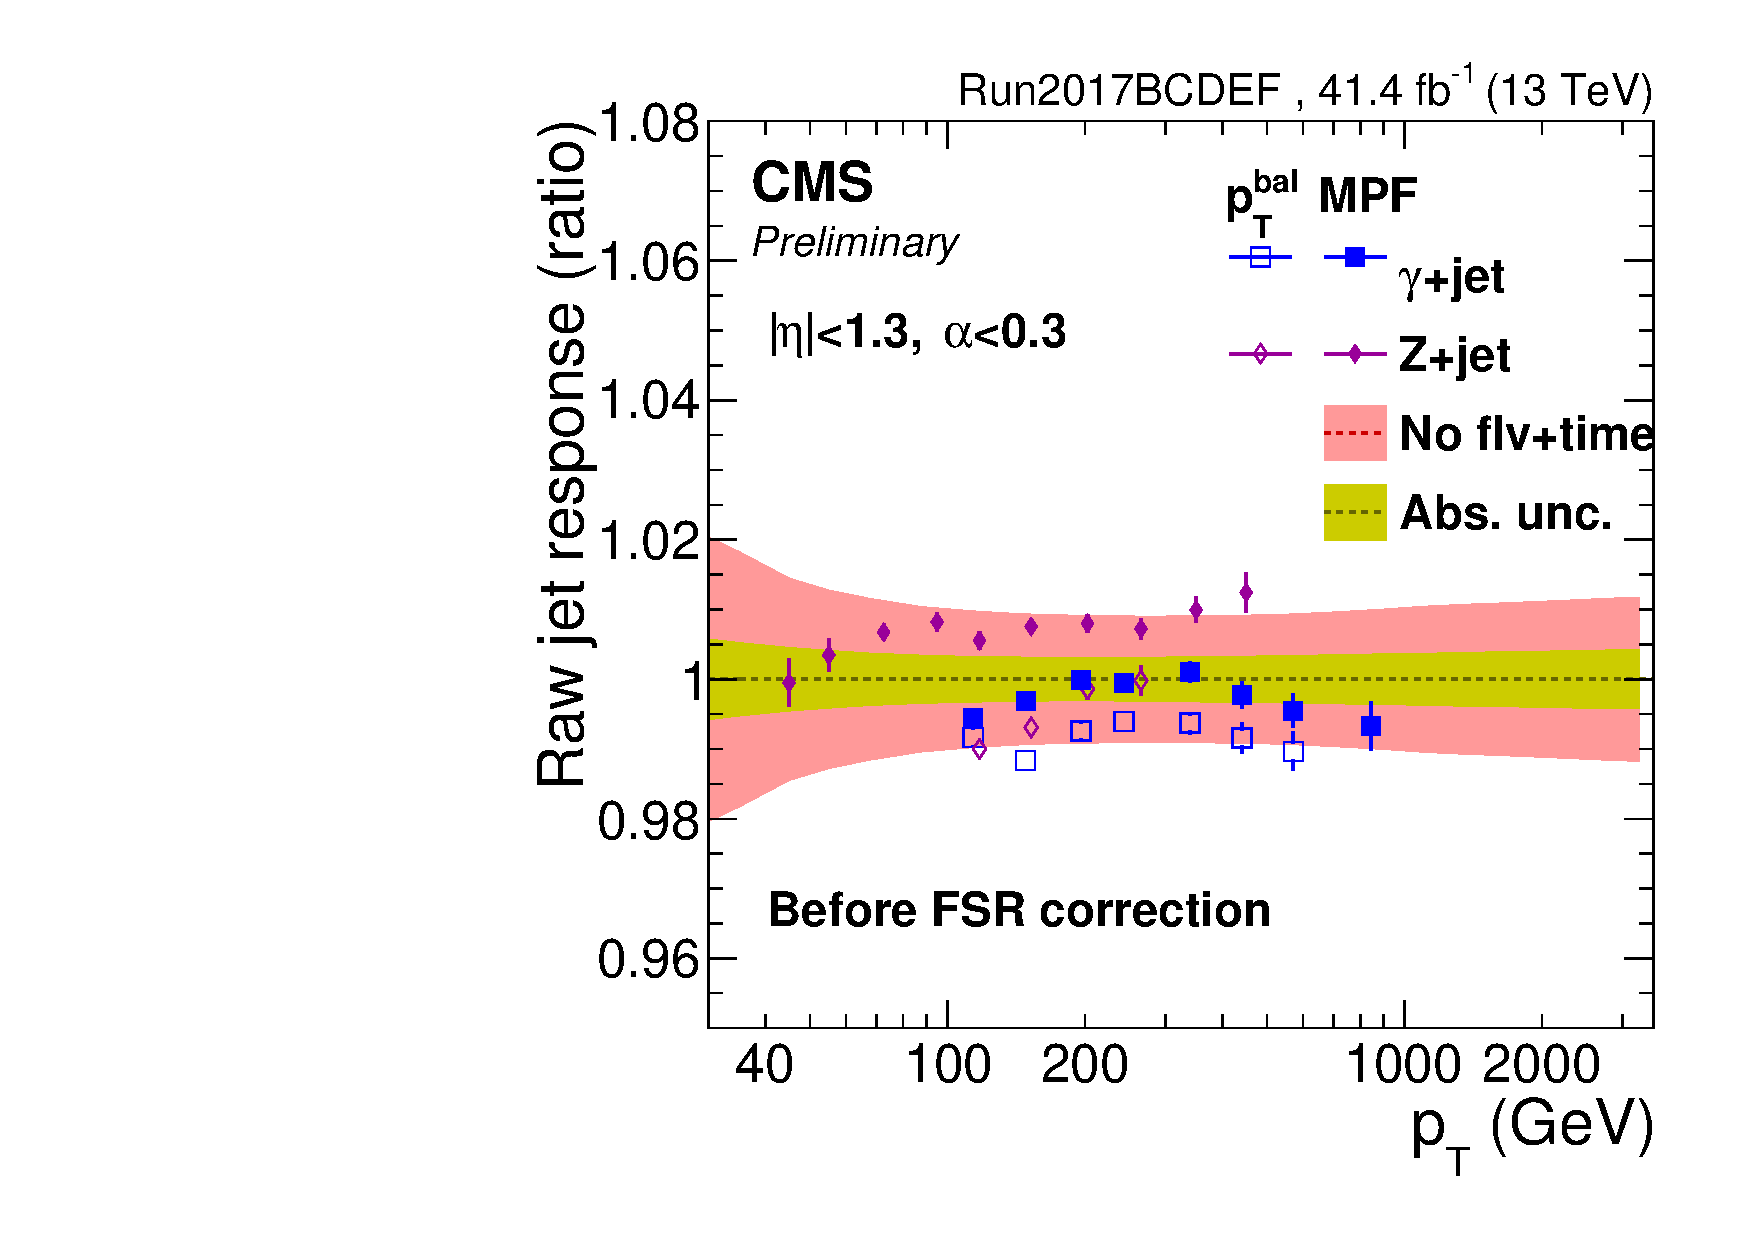
\includegraphics[width=0.32\textwidth]{\RunPeriod/globalFitL3res_raw.pdf}
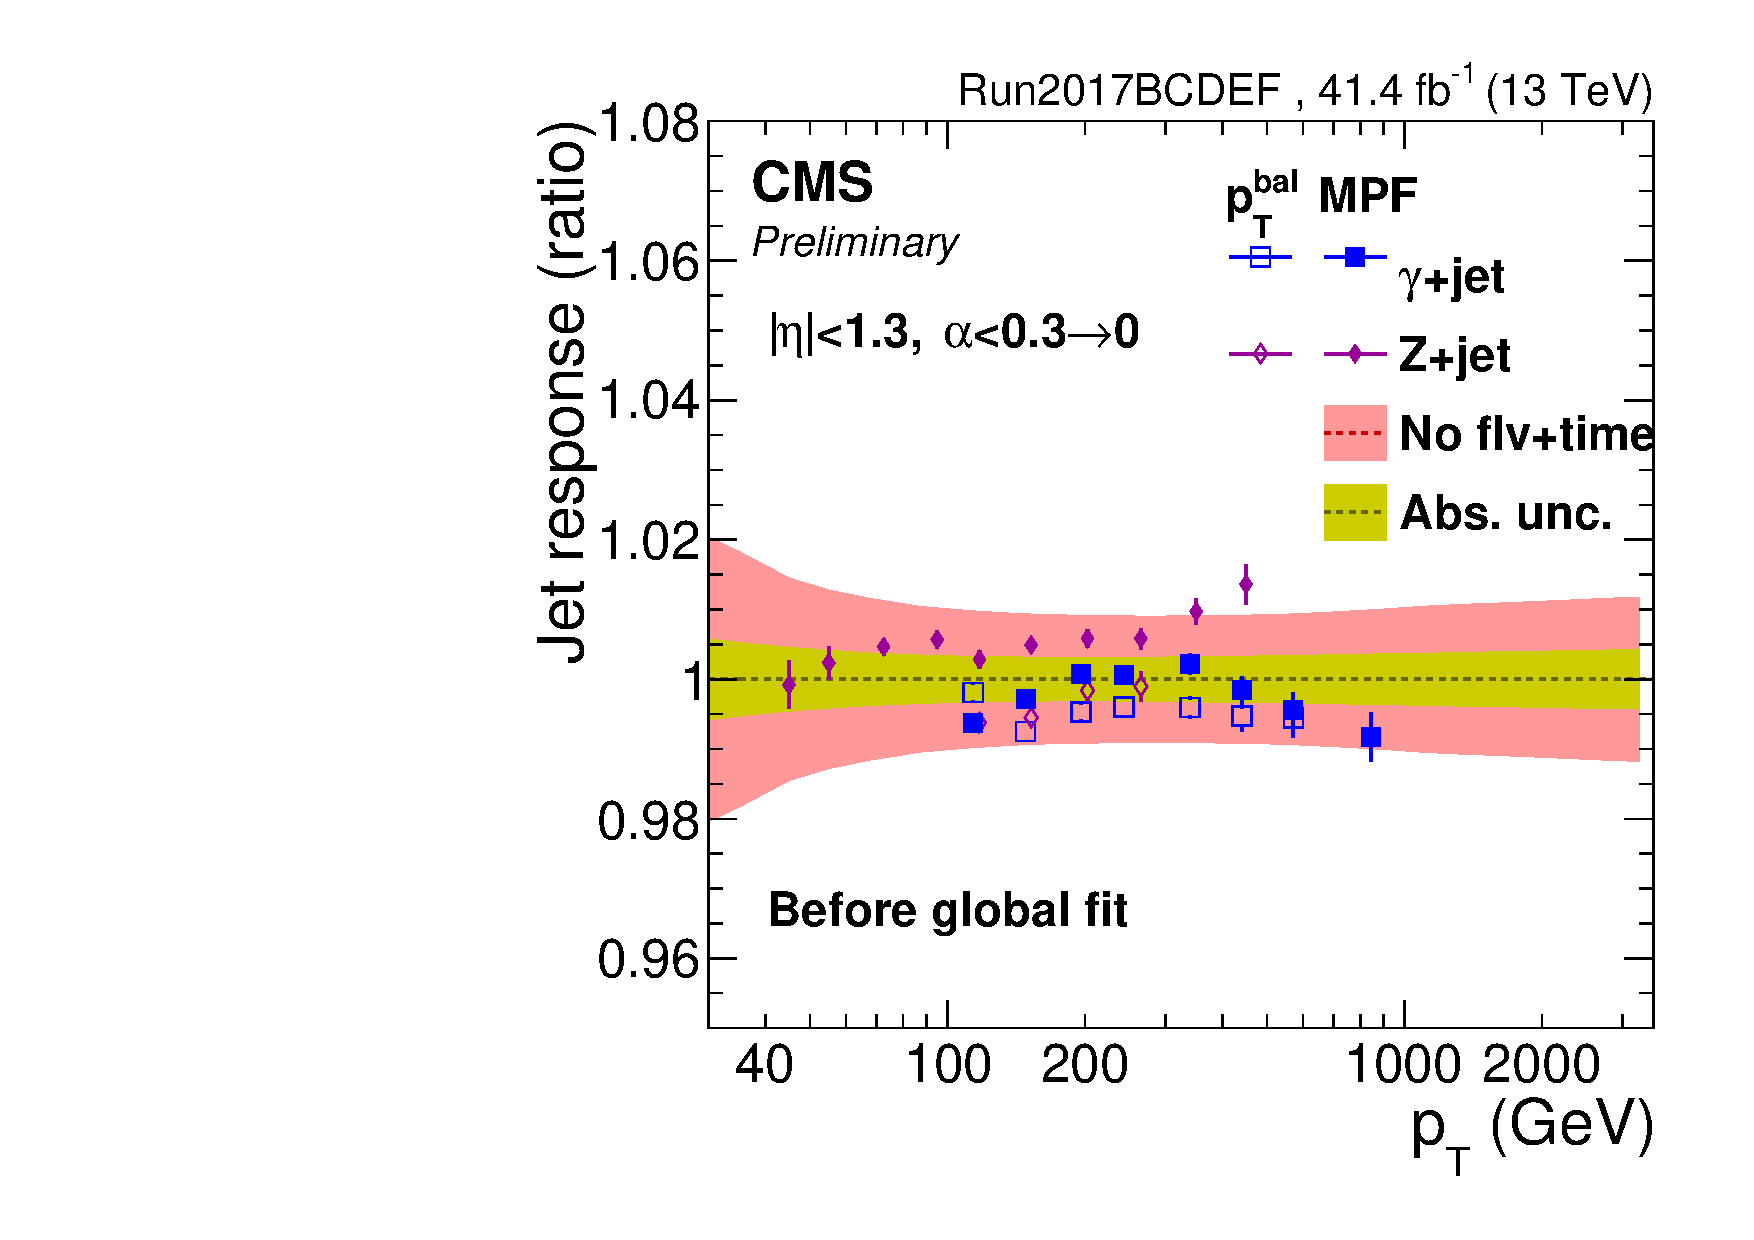
\includegraphics[width=0.32\textwidth]{\RunPeriod/globalFitL3res_orig.pdf}
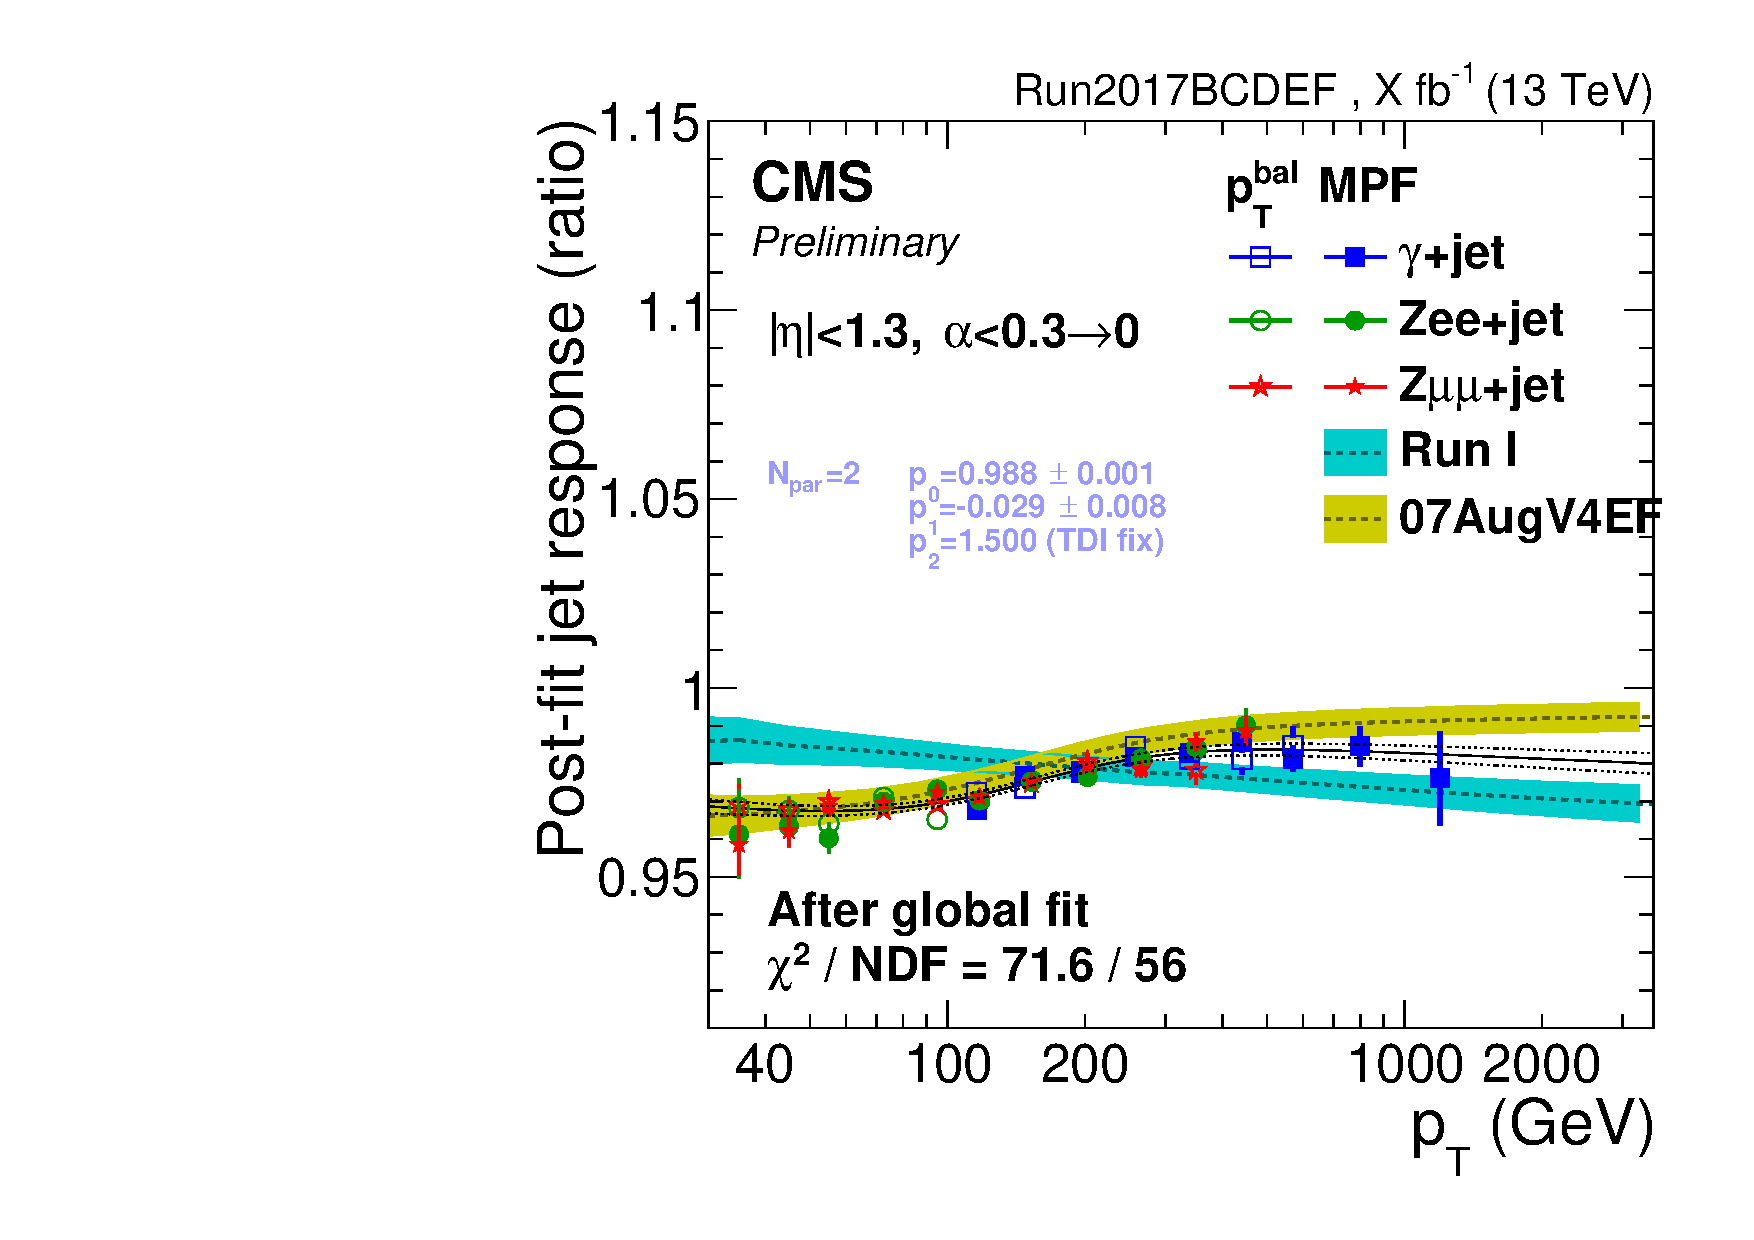
\includegraphics[width=0.32\textwidth]{\RunPeriod/globalFitL3res_shifted.pdf}\\
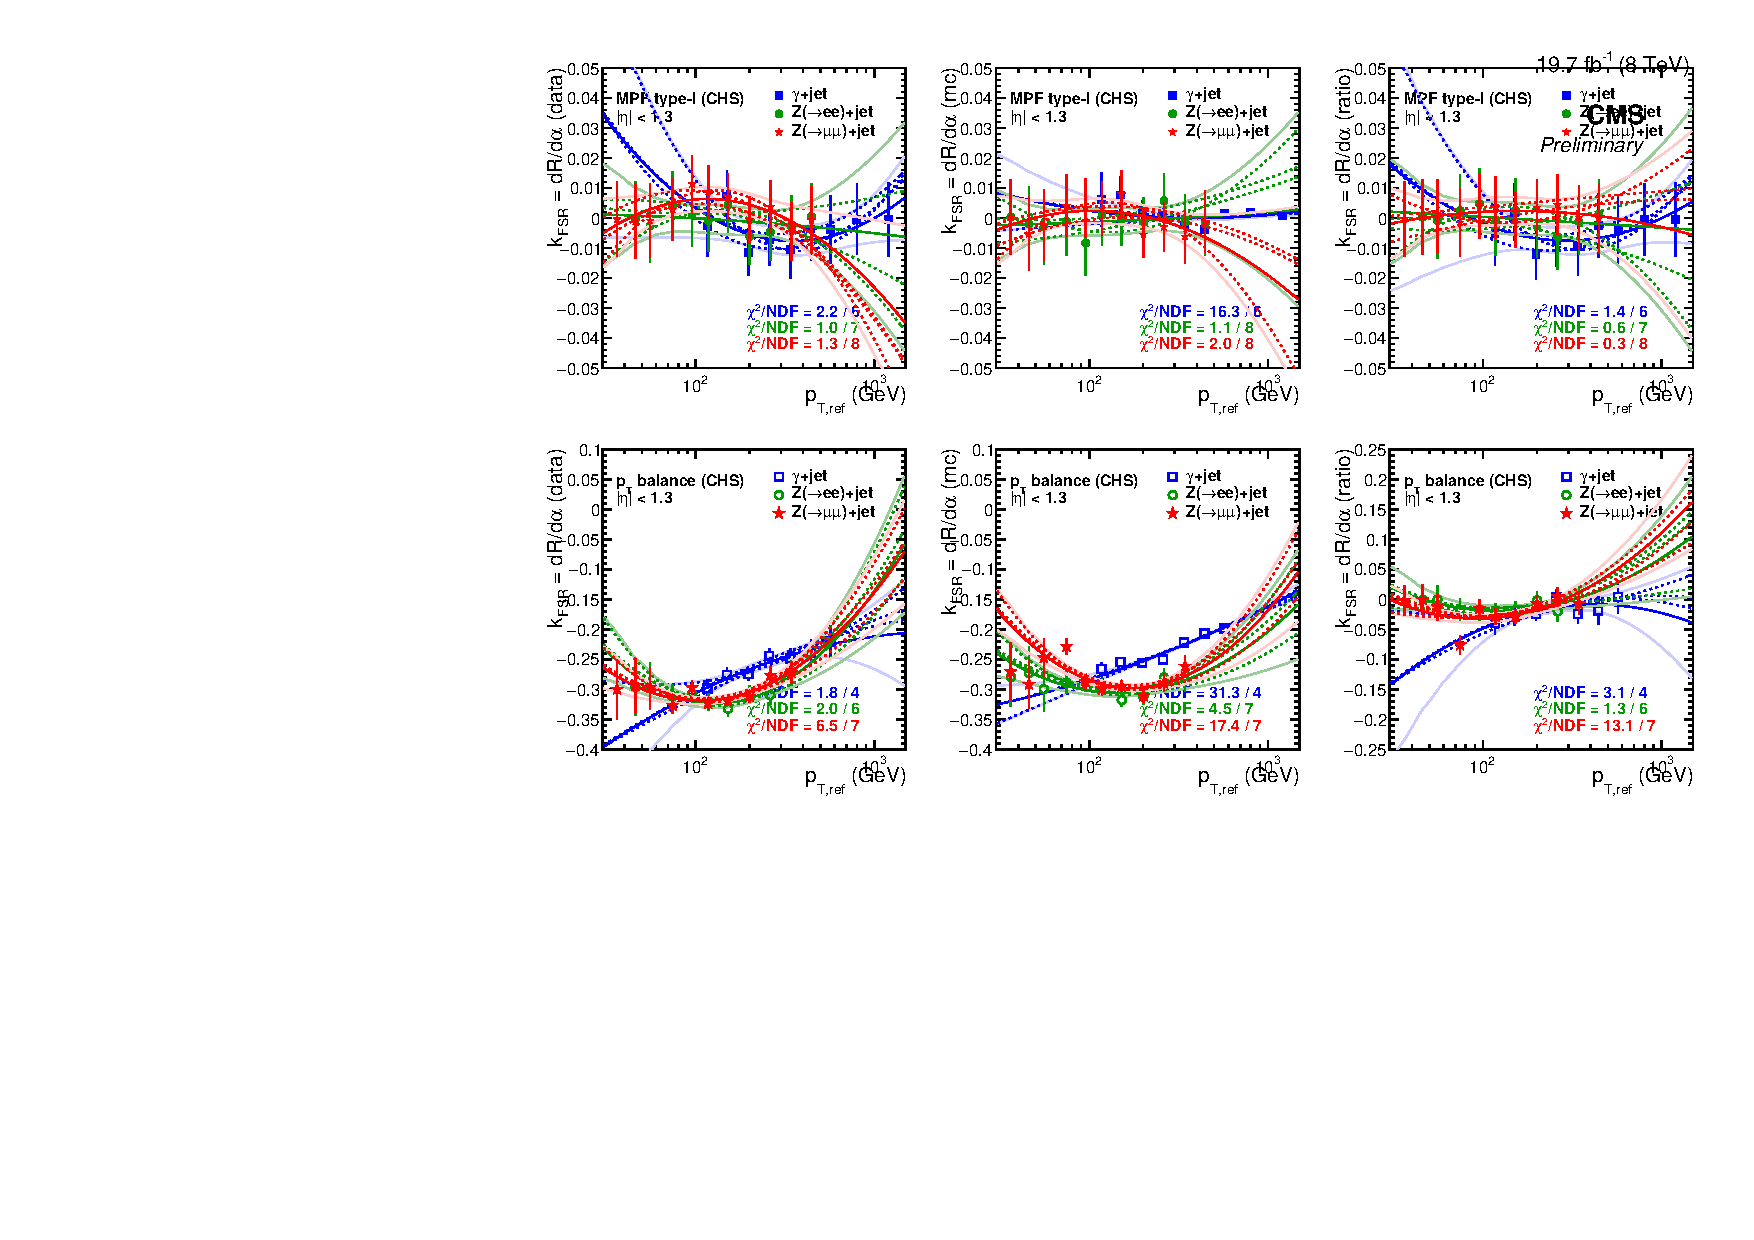
\includegraphics[width=0.30\textwidth]{\RunPeriod/softrad_2x6_kfsr_eta00-13.pdf}
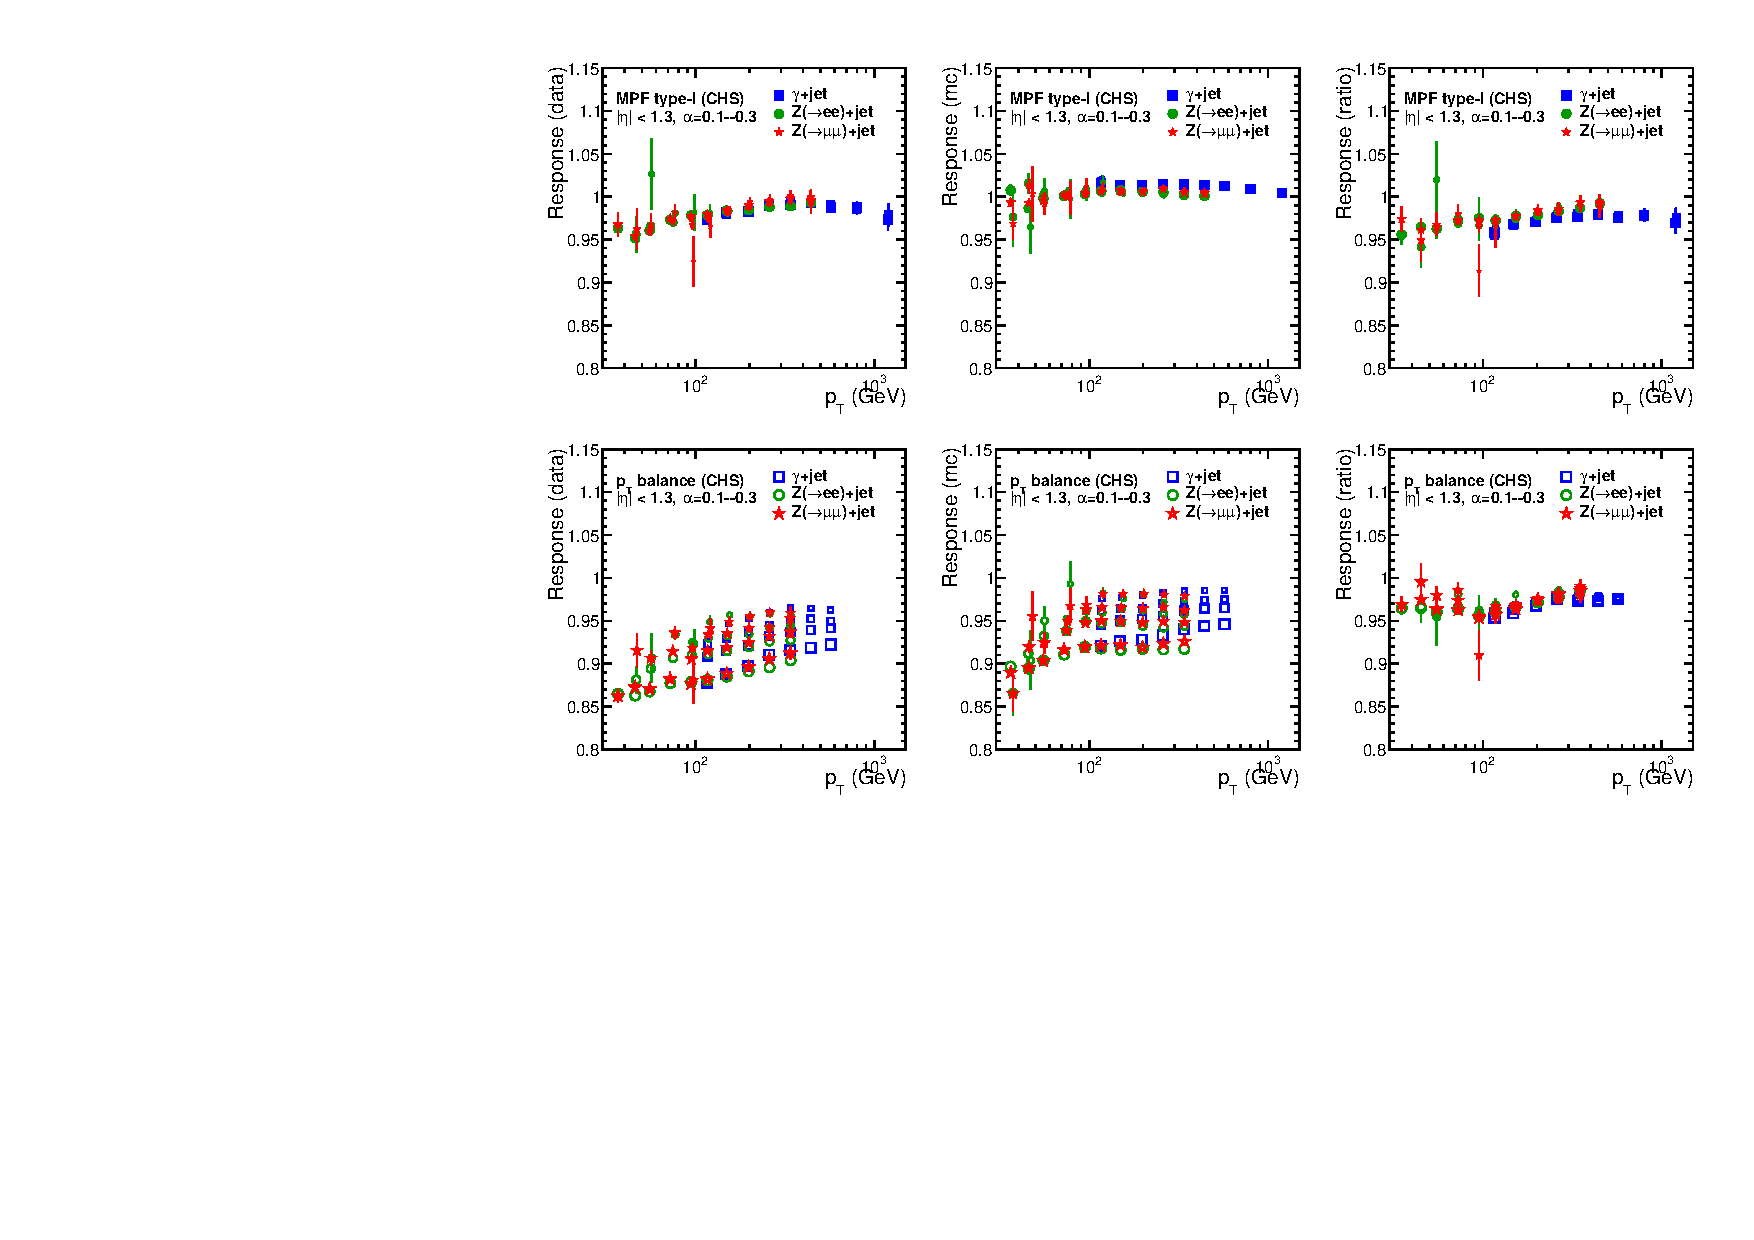
\includegraphics[width=0.30\textwidth]{\RunPeriod/softrad_2x6_vspt_eta00-13.pdf}
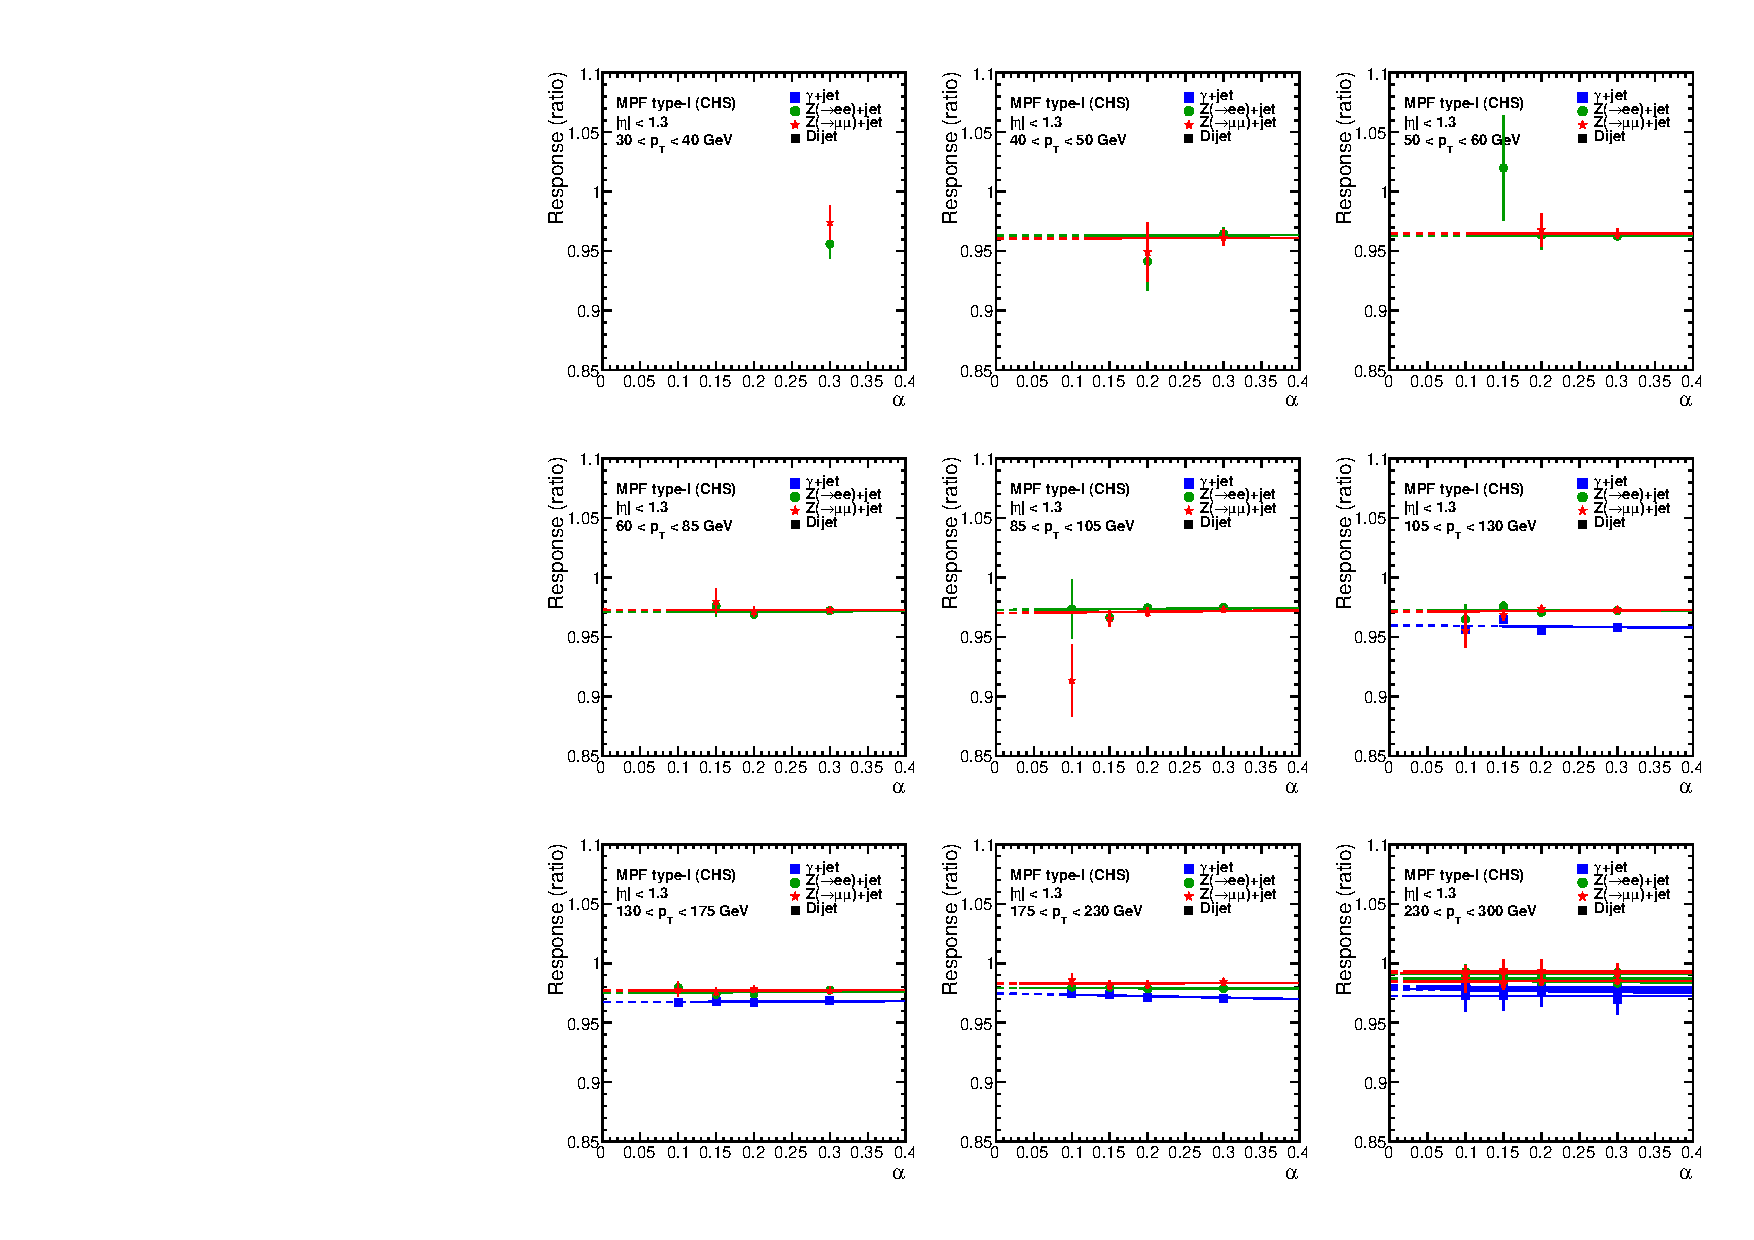
\includegraphics[width=0.20\textwidth]{\RunPeriod/softrad_3x3_ratio_mpfchs1_vsalpha_eta00-13.pdf}
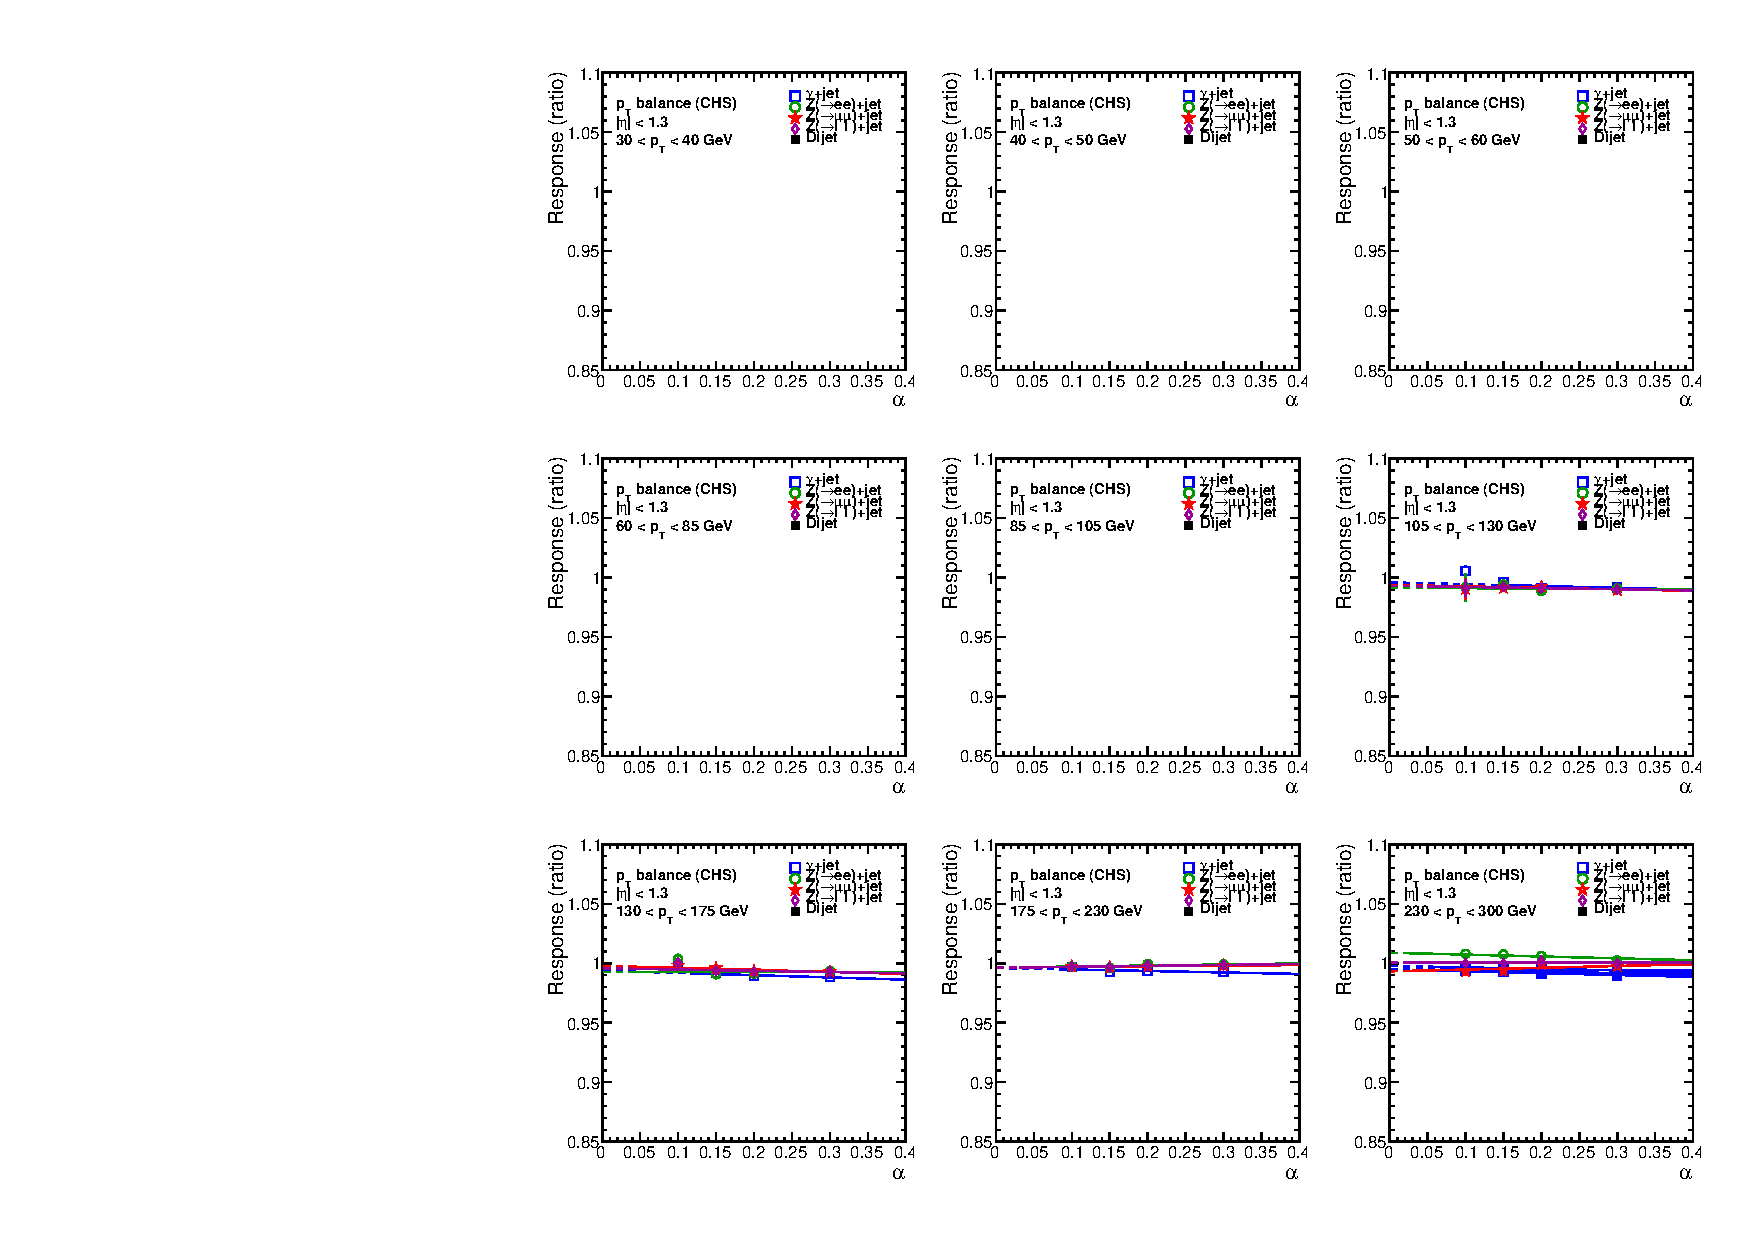
\includegraphics[width=0.20\textwidth]{\RunPeriod/softrad_3x3_ratio_ptchs_vsalpha_eta00-13.pdf}\\

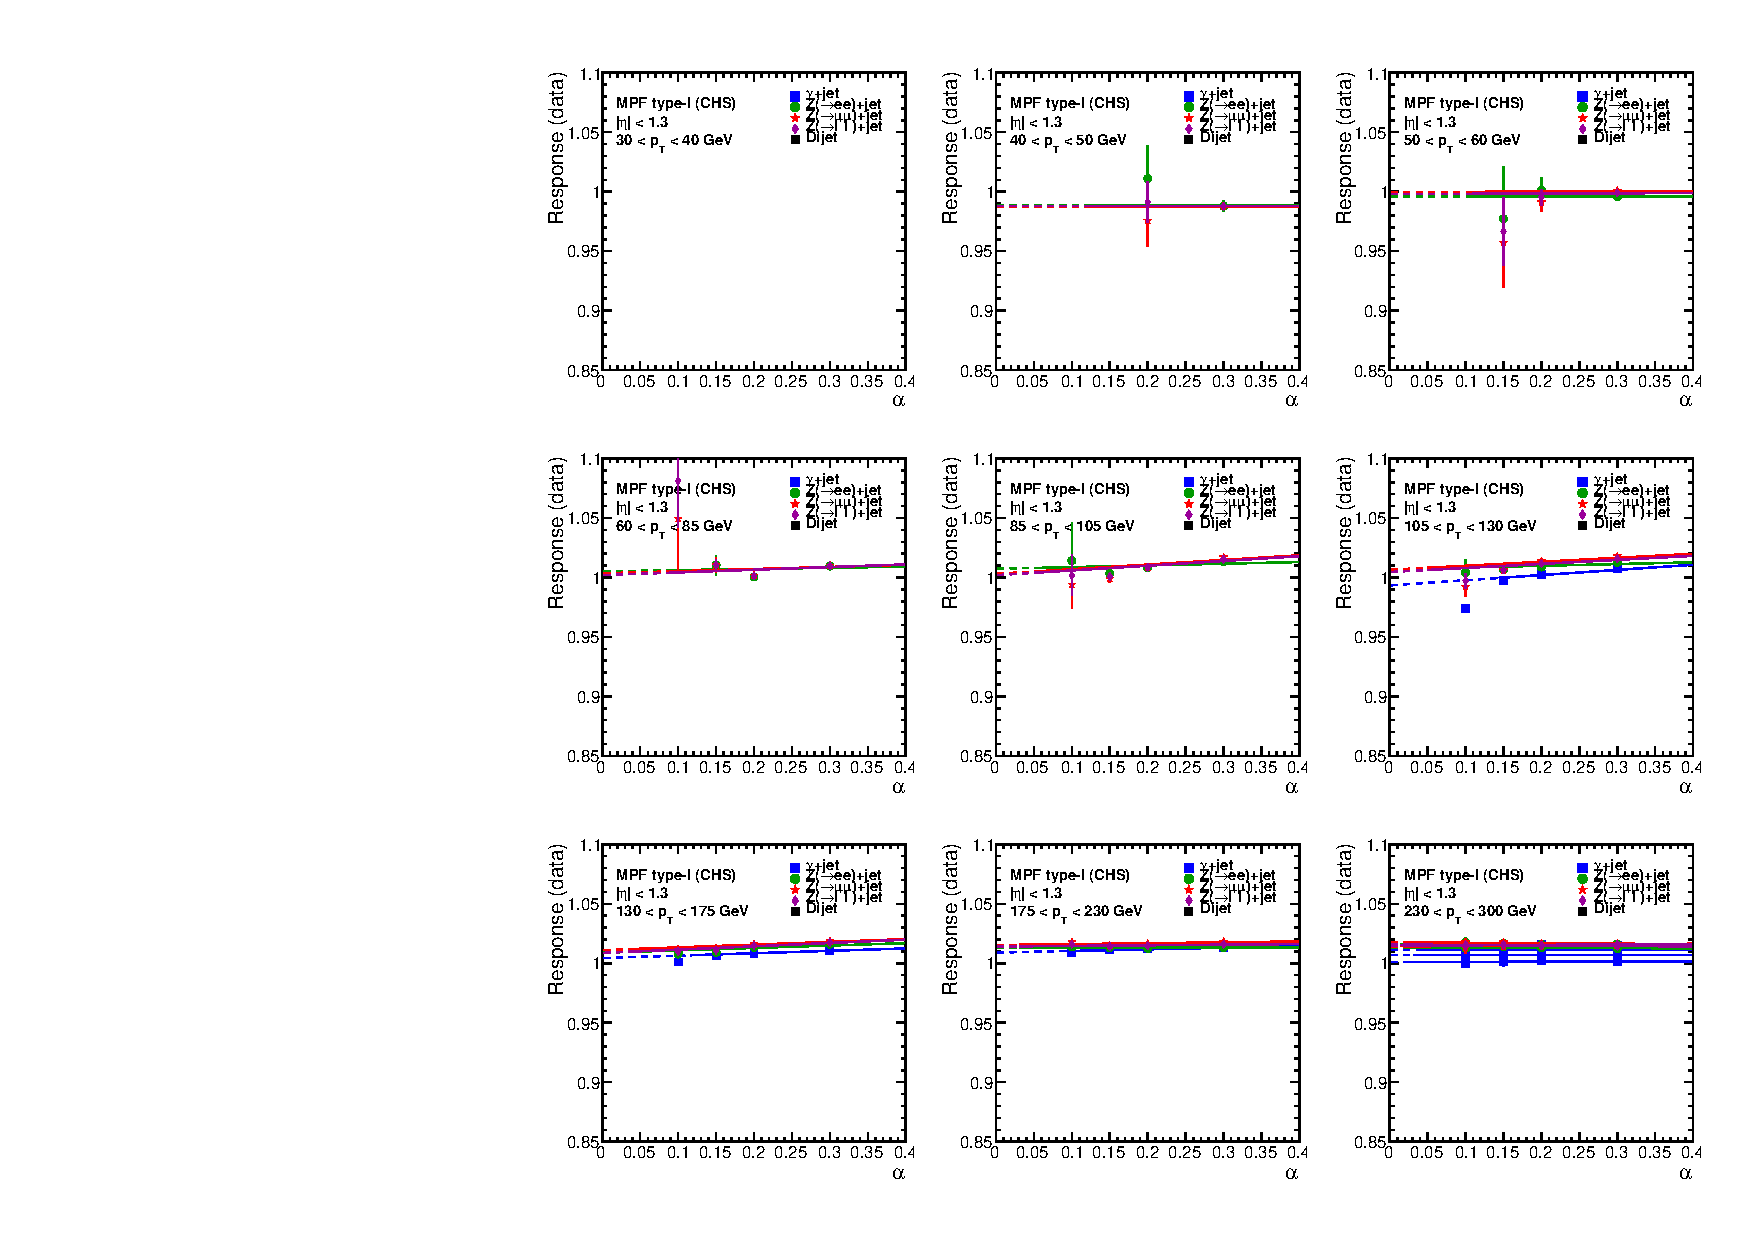
\includegraphics[width=0.15\textwidth]{\RunPeriod/softrad_3x3_data_mpfchs1_vsalpha_eta00-13.pdf}
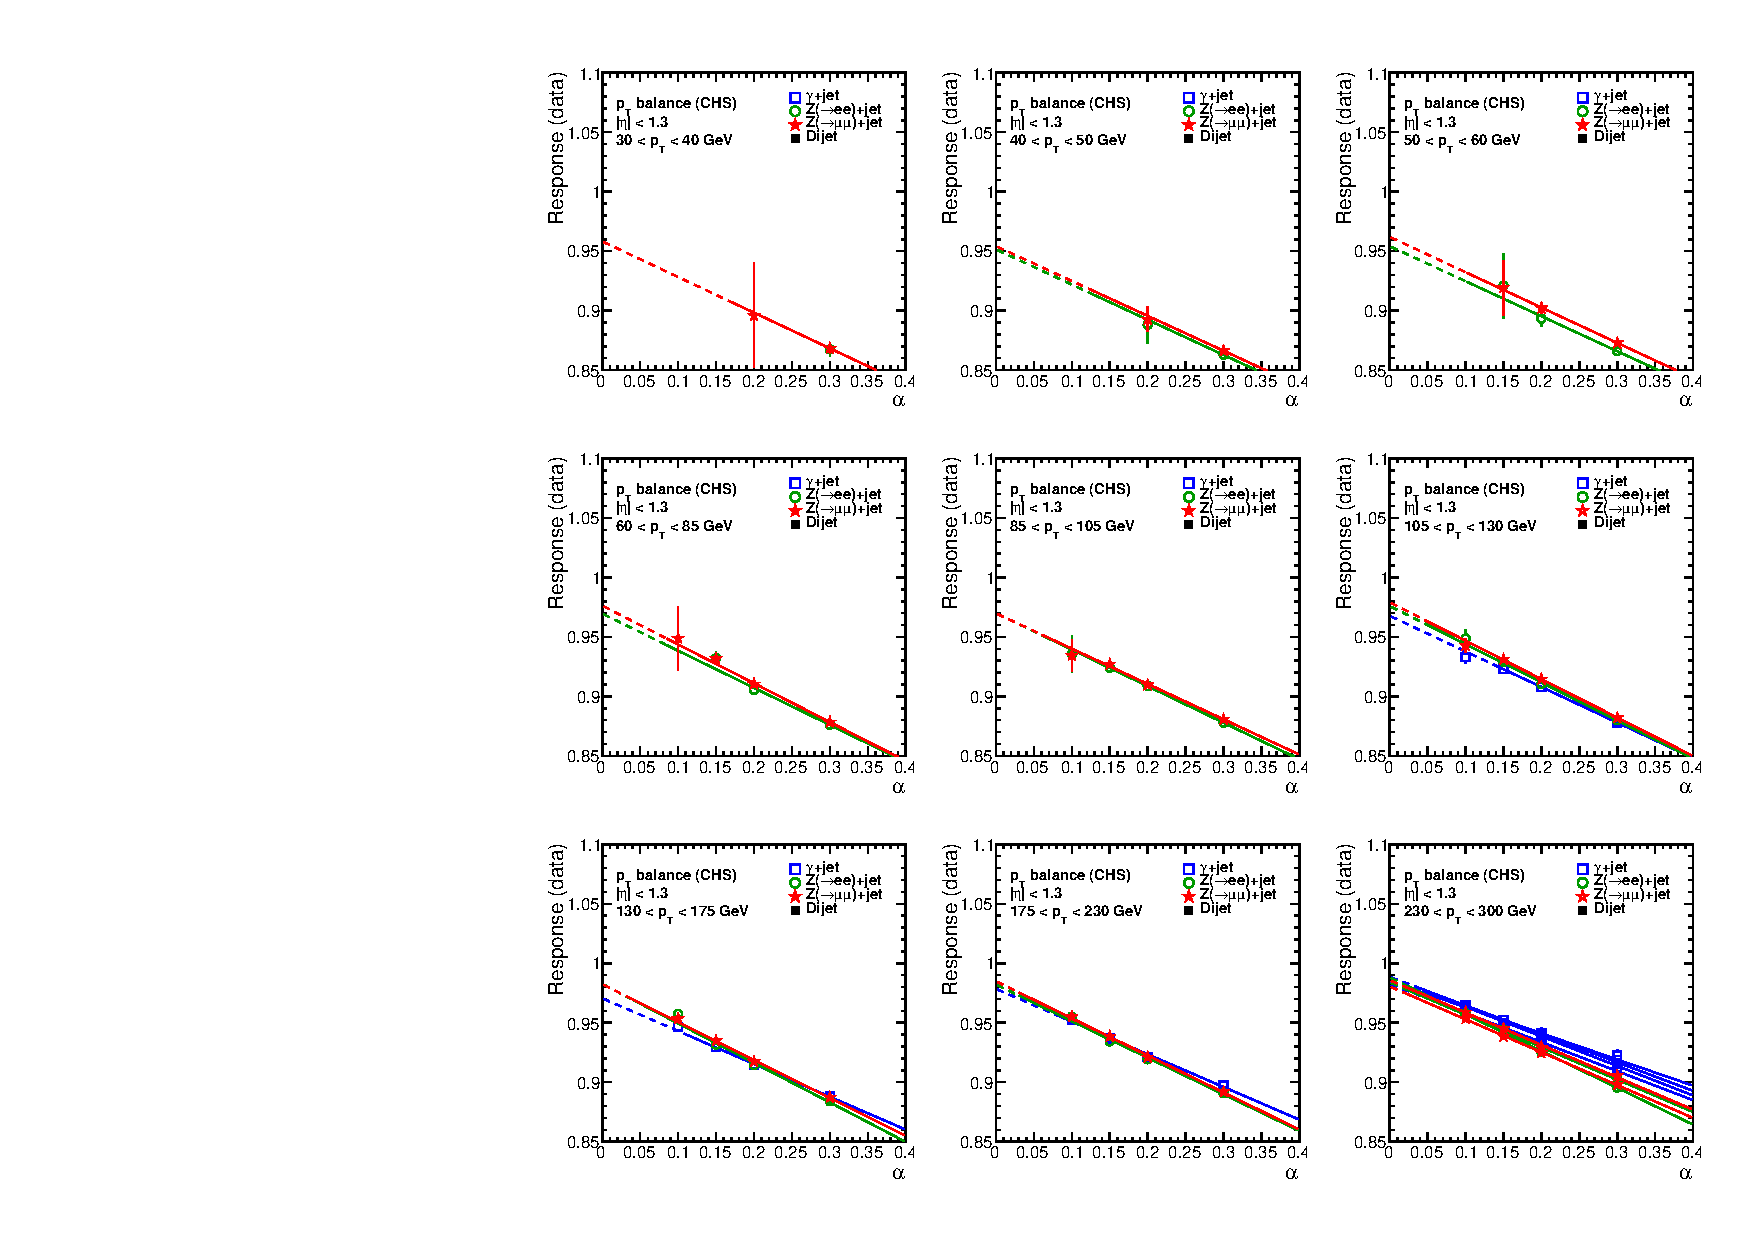
\includegraphics[width=0.15\textwidth]{\RunPeriod/softrad_3x3_data_ptchs_vsalpha_eta00-13.pdf}
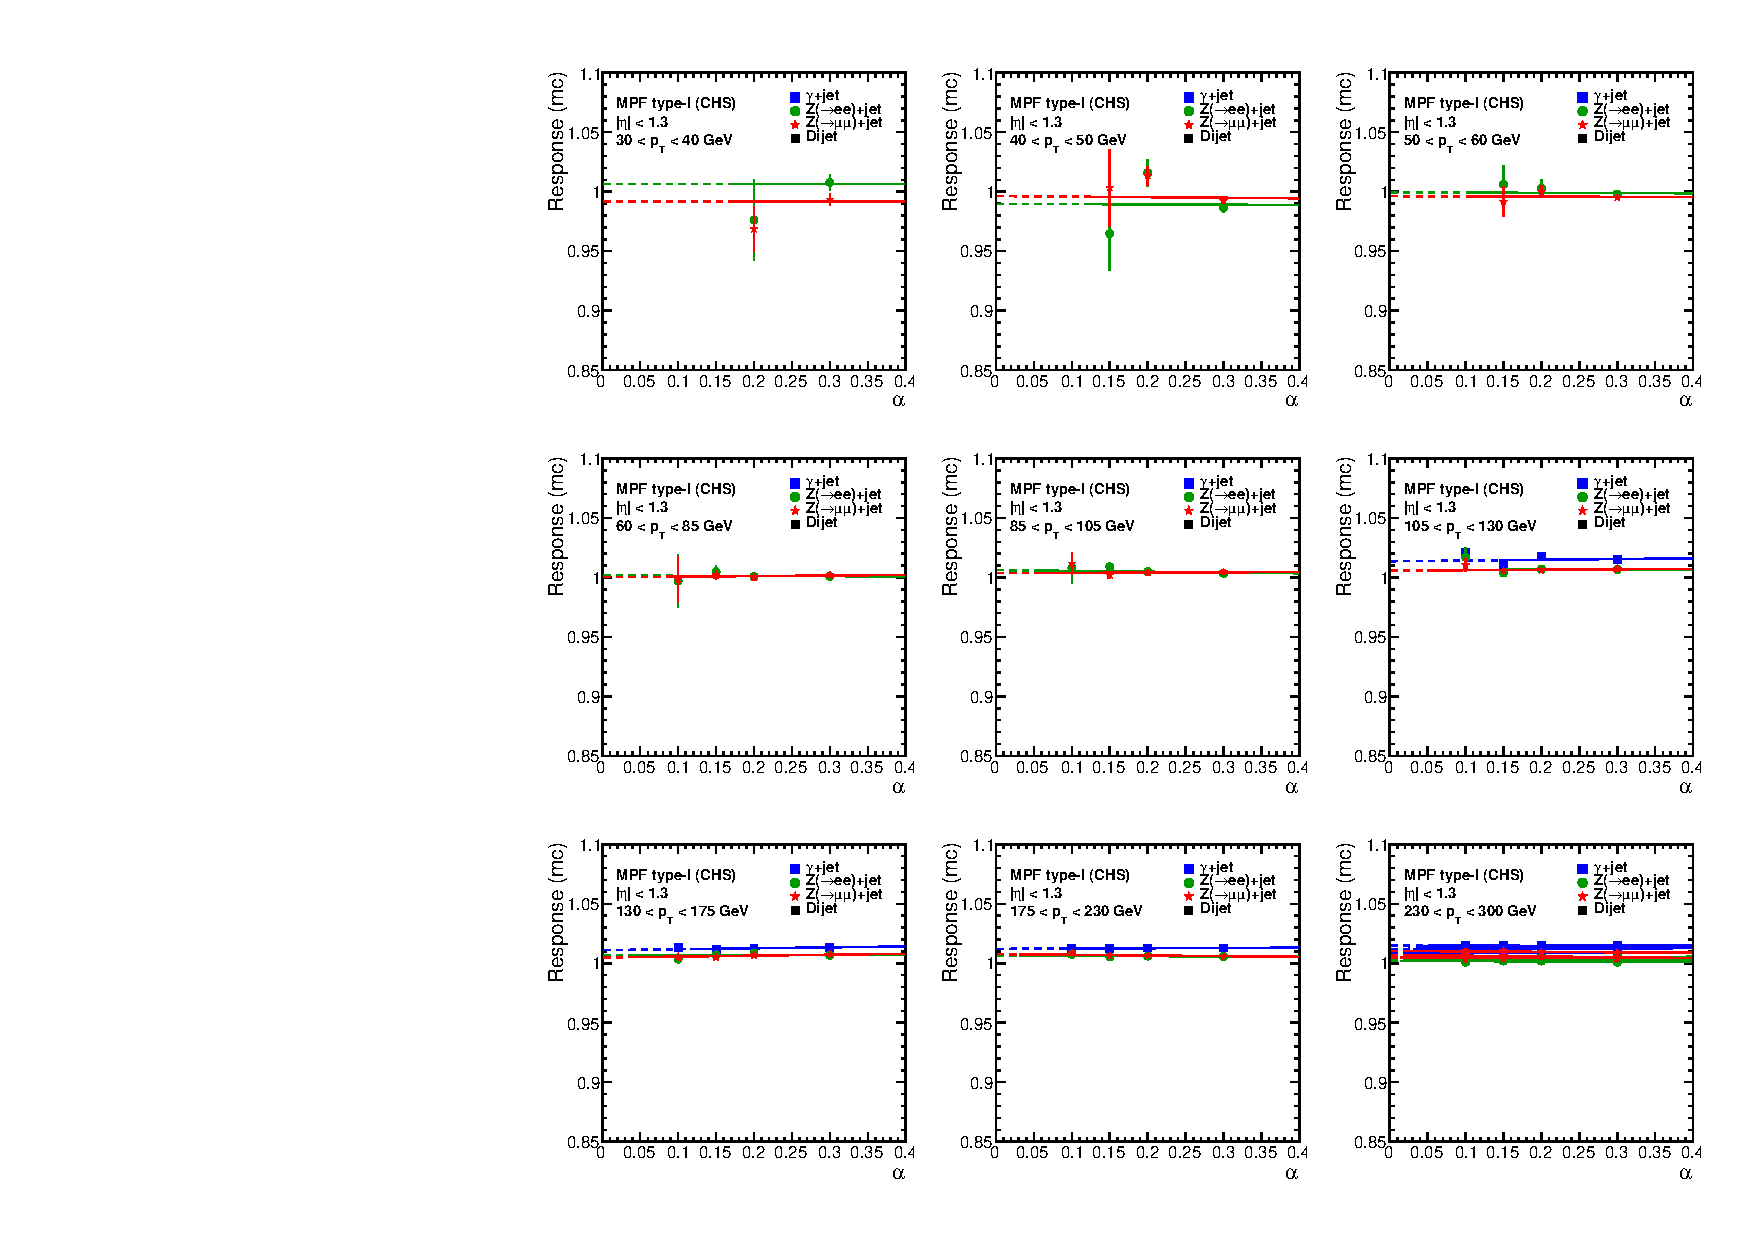
\includegraphics[width=0.15\textwidth]{\RunPeriod/softrad_3x3_mc_mpfchs1_vsalpha_eta00-13.pdf} 
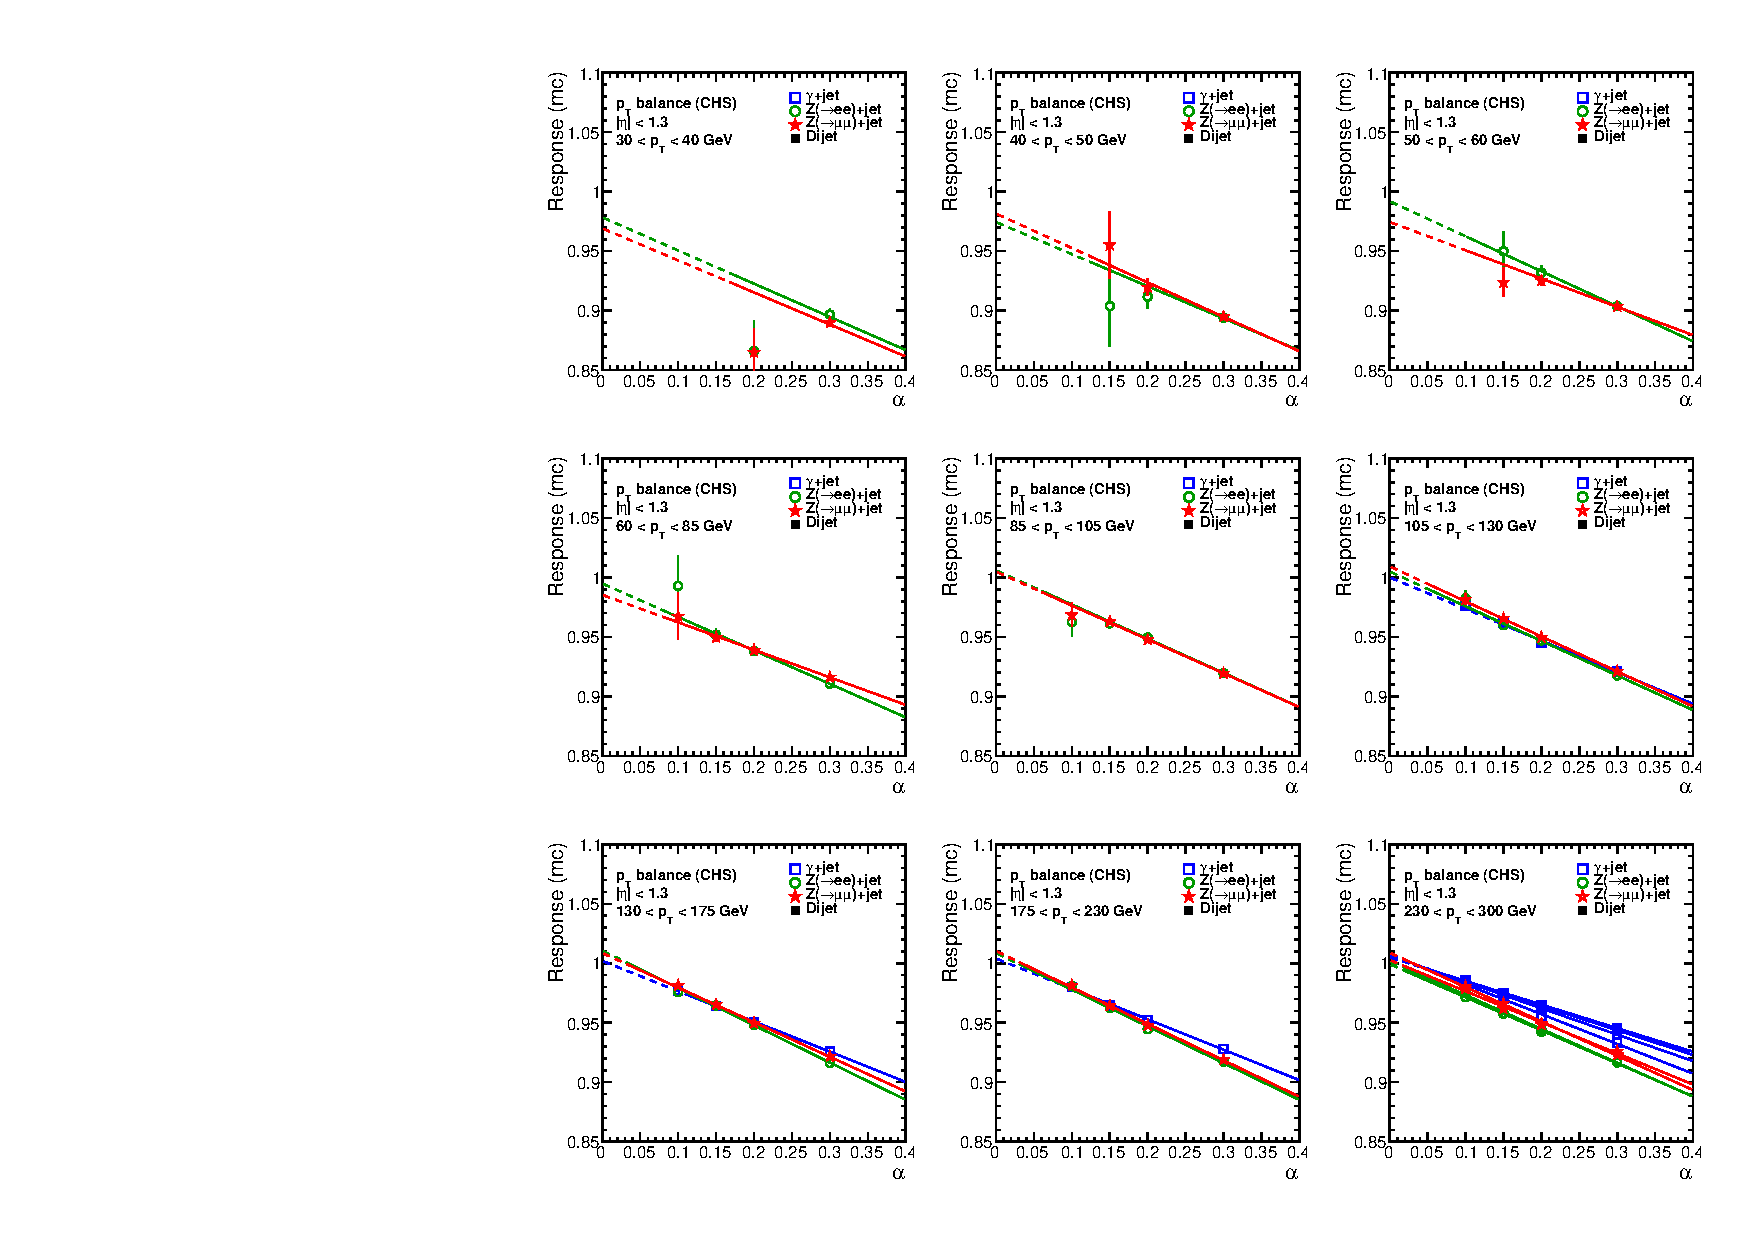
\includegraphics[width=0.15\textwidth]{\RunPeriod/softrad_3x3_mc_ptchs_vsalpha_eta00-13.pdf}  
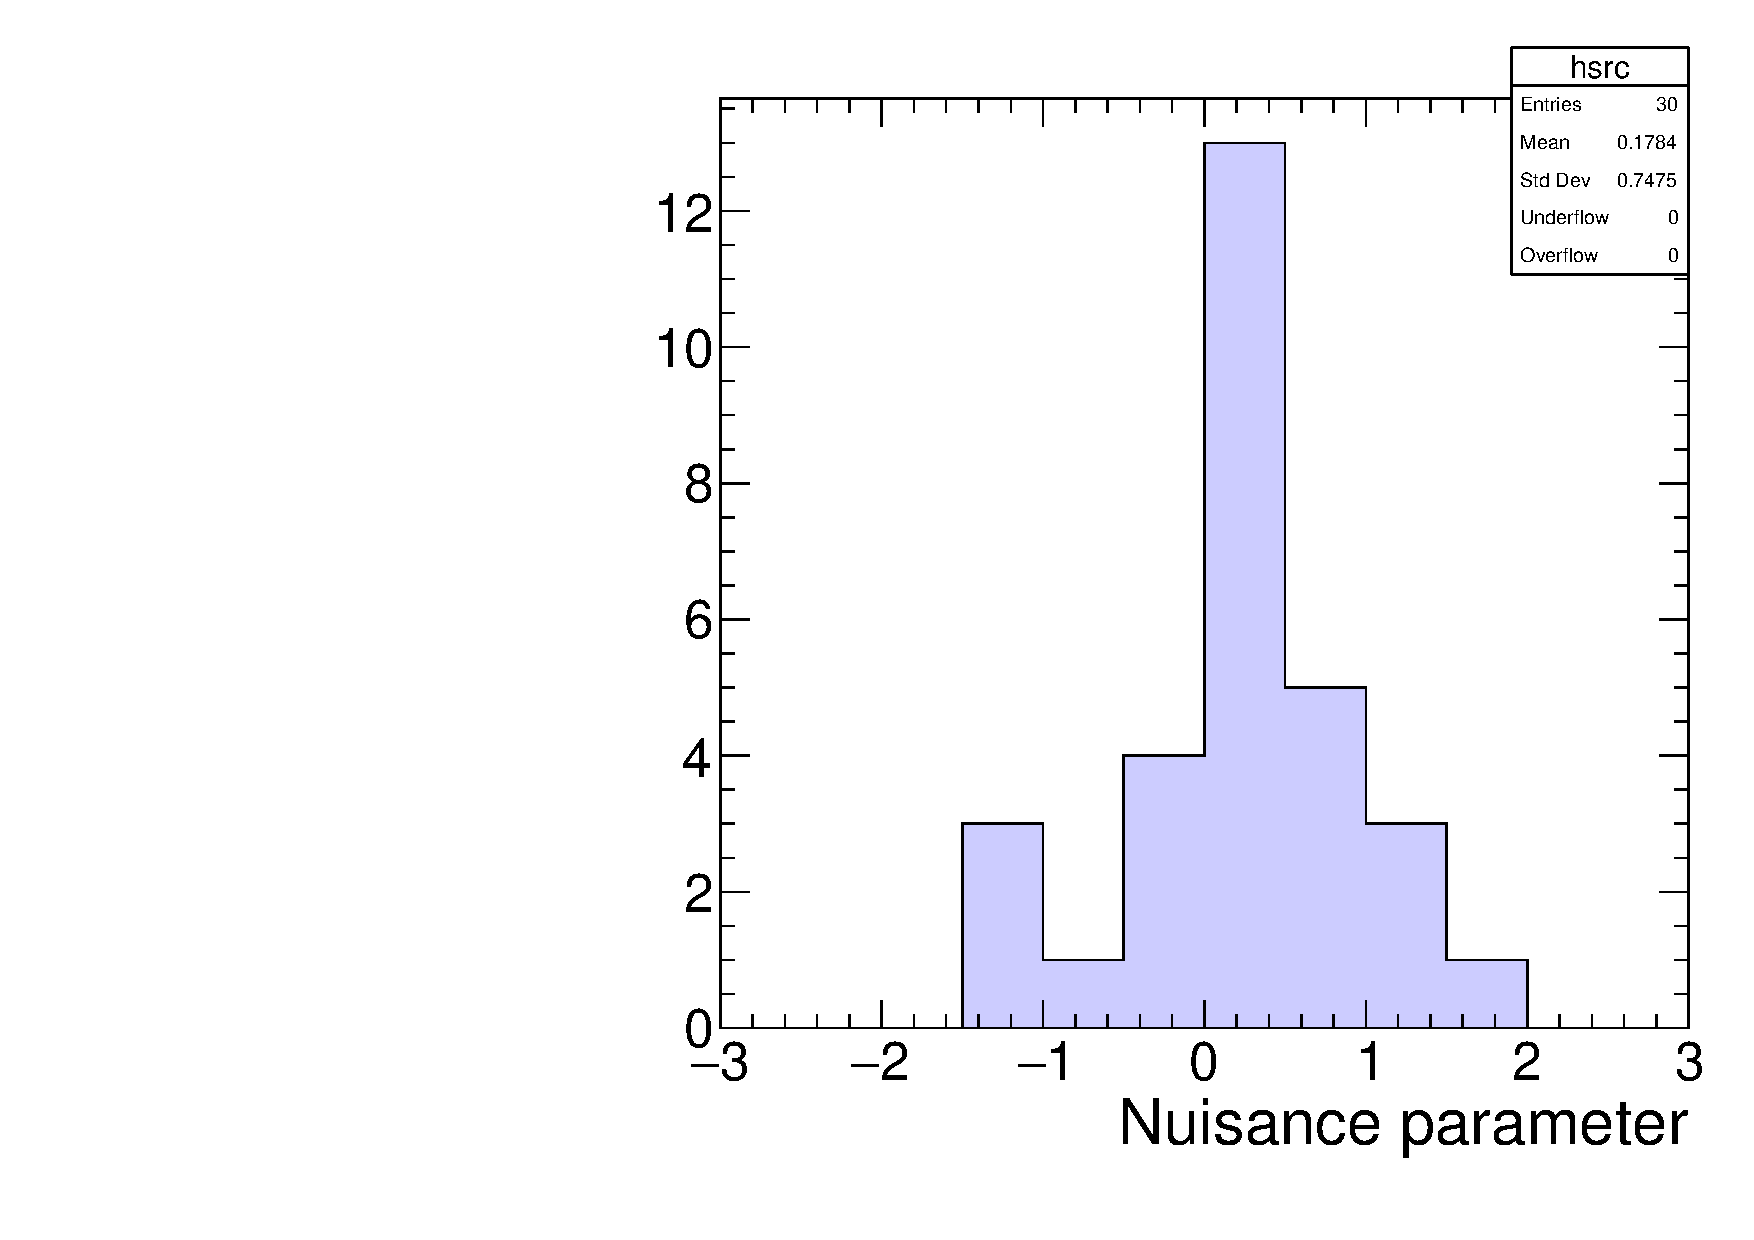
\includegraphics[width=0.10\textwidth]{\RunPeriod/globalFitL3res_hsrc.pdf}
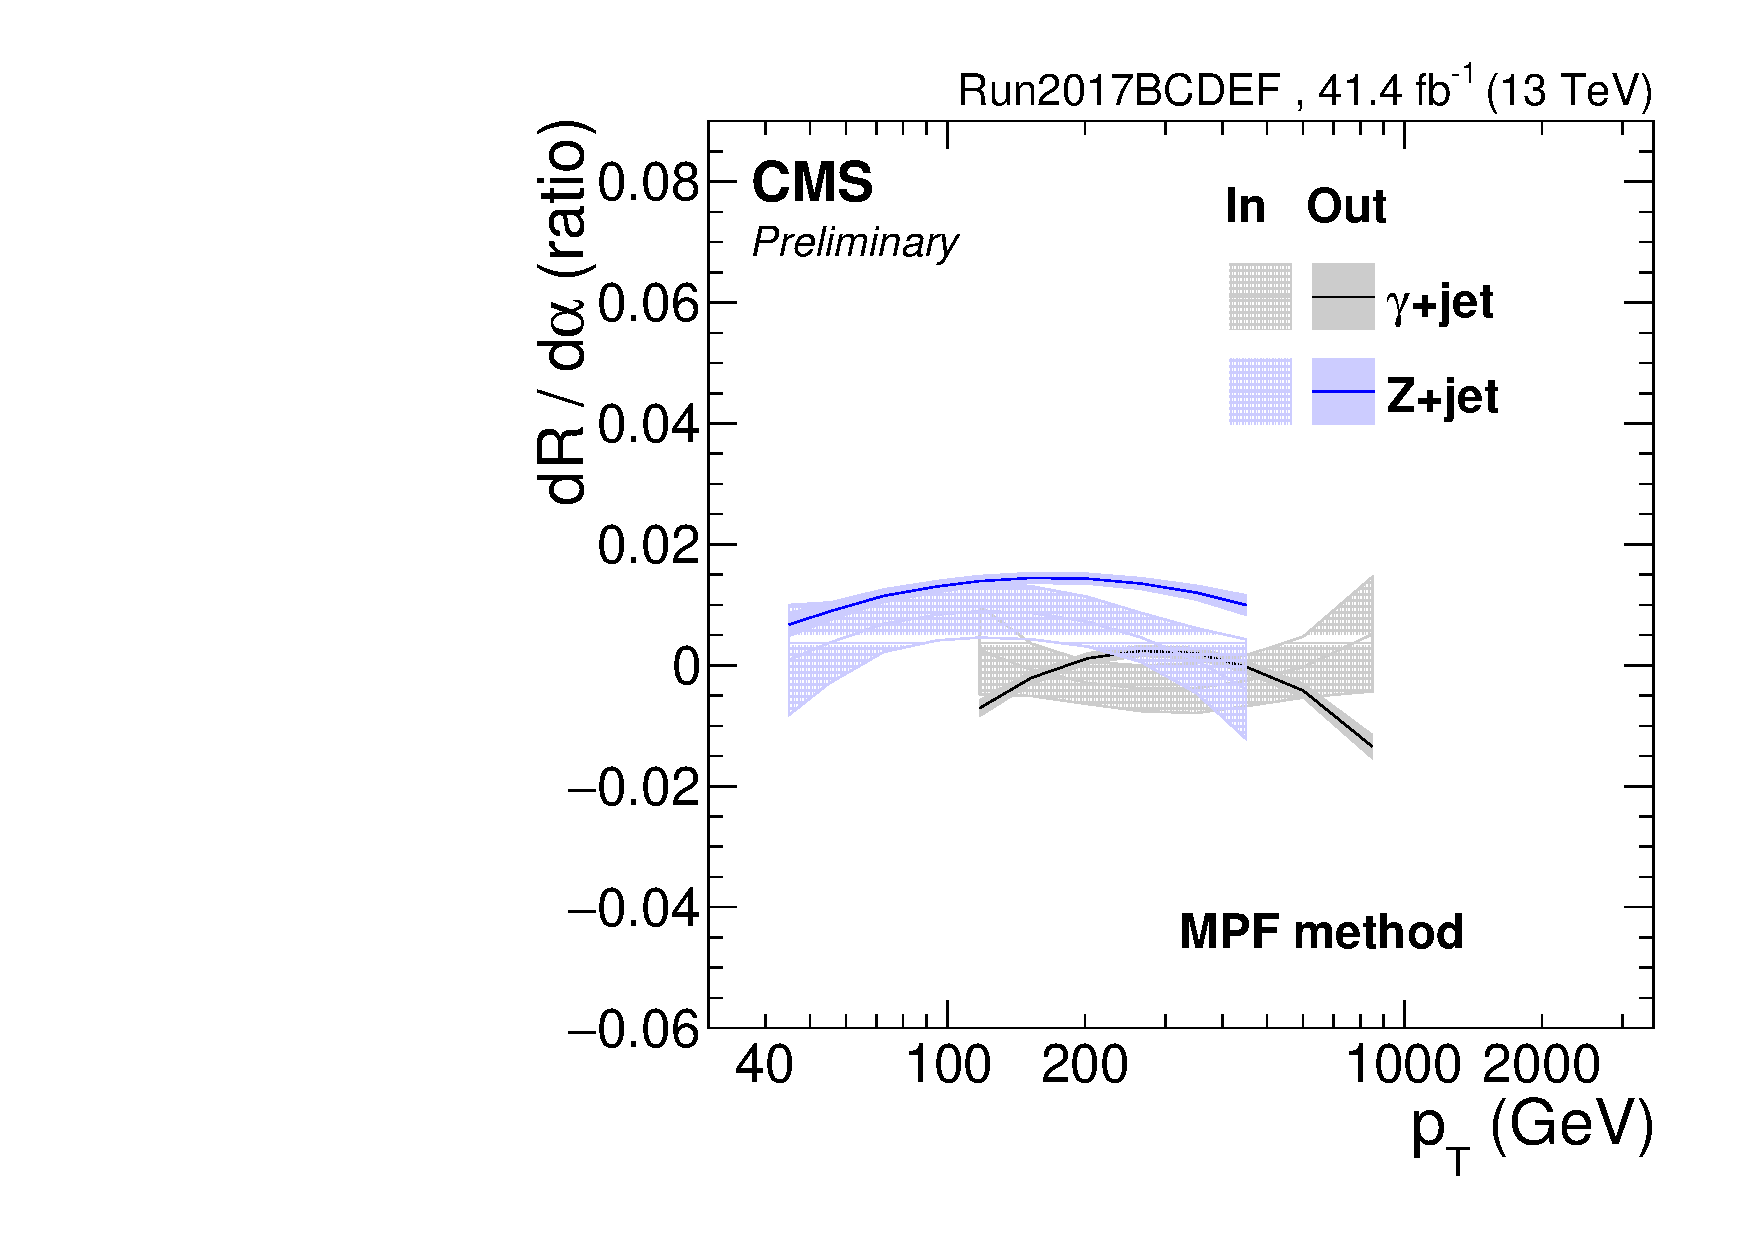
\includegraphics[width=0.10\textwidth]{\RunPeriod/globalFitL3res_mpfchs1_kfsr.pdf}
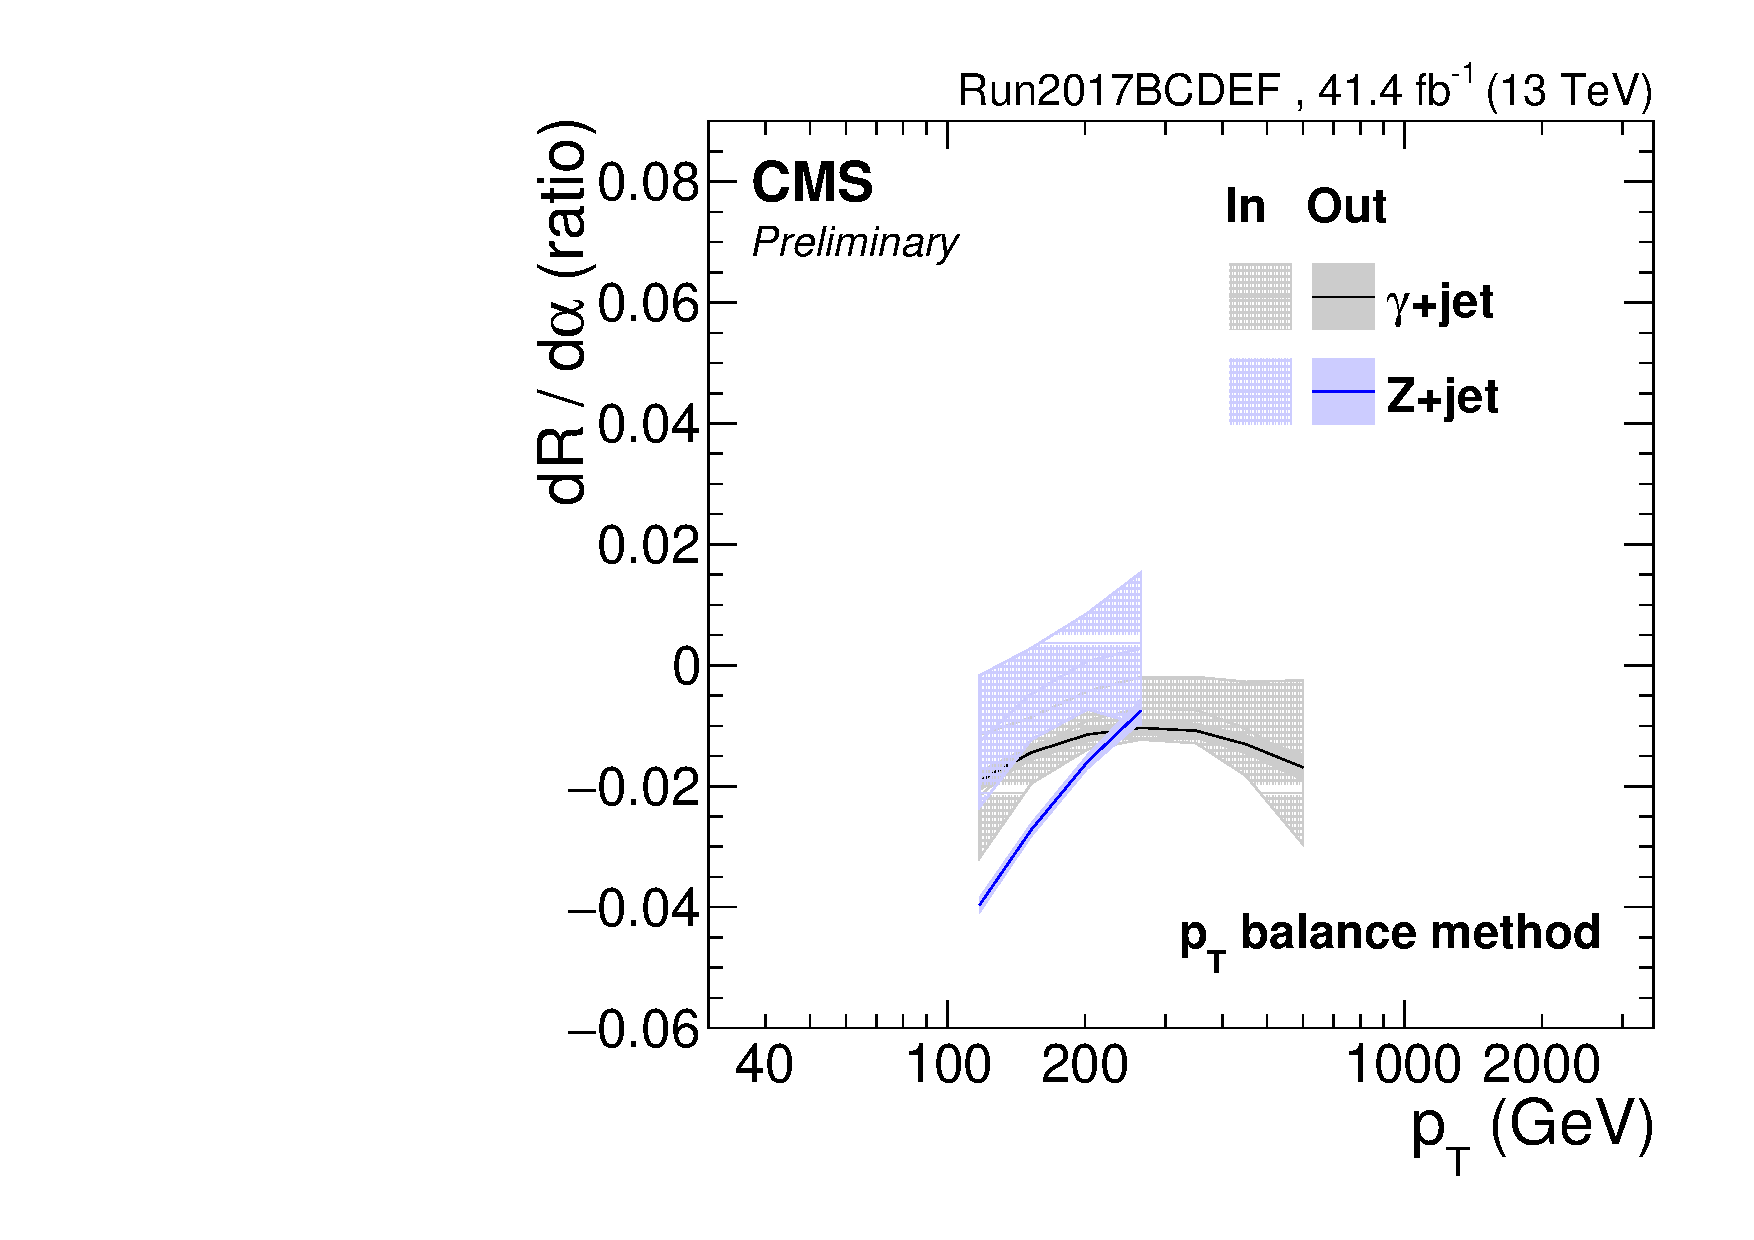
\includegraphics[width=0.10\textwidth]{\RunPeriod/globalFitL3res_ptchs_kfsr.pdf}\\

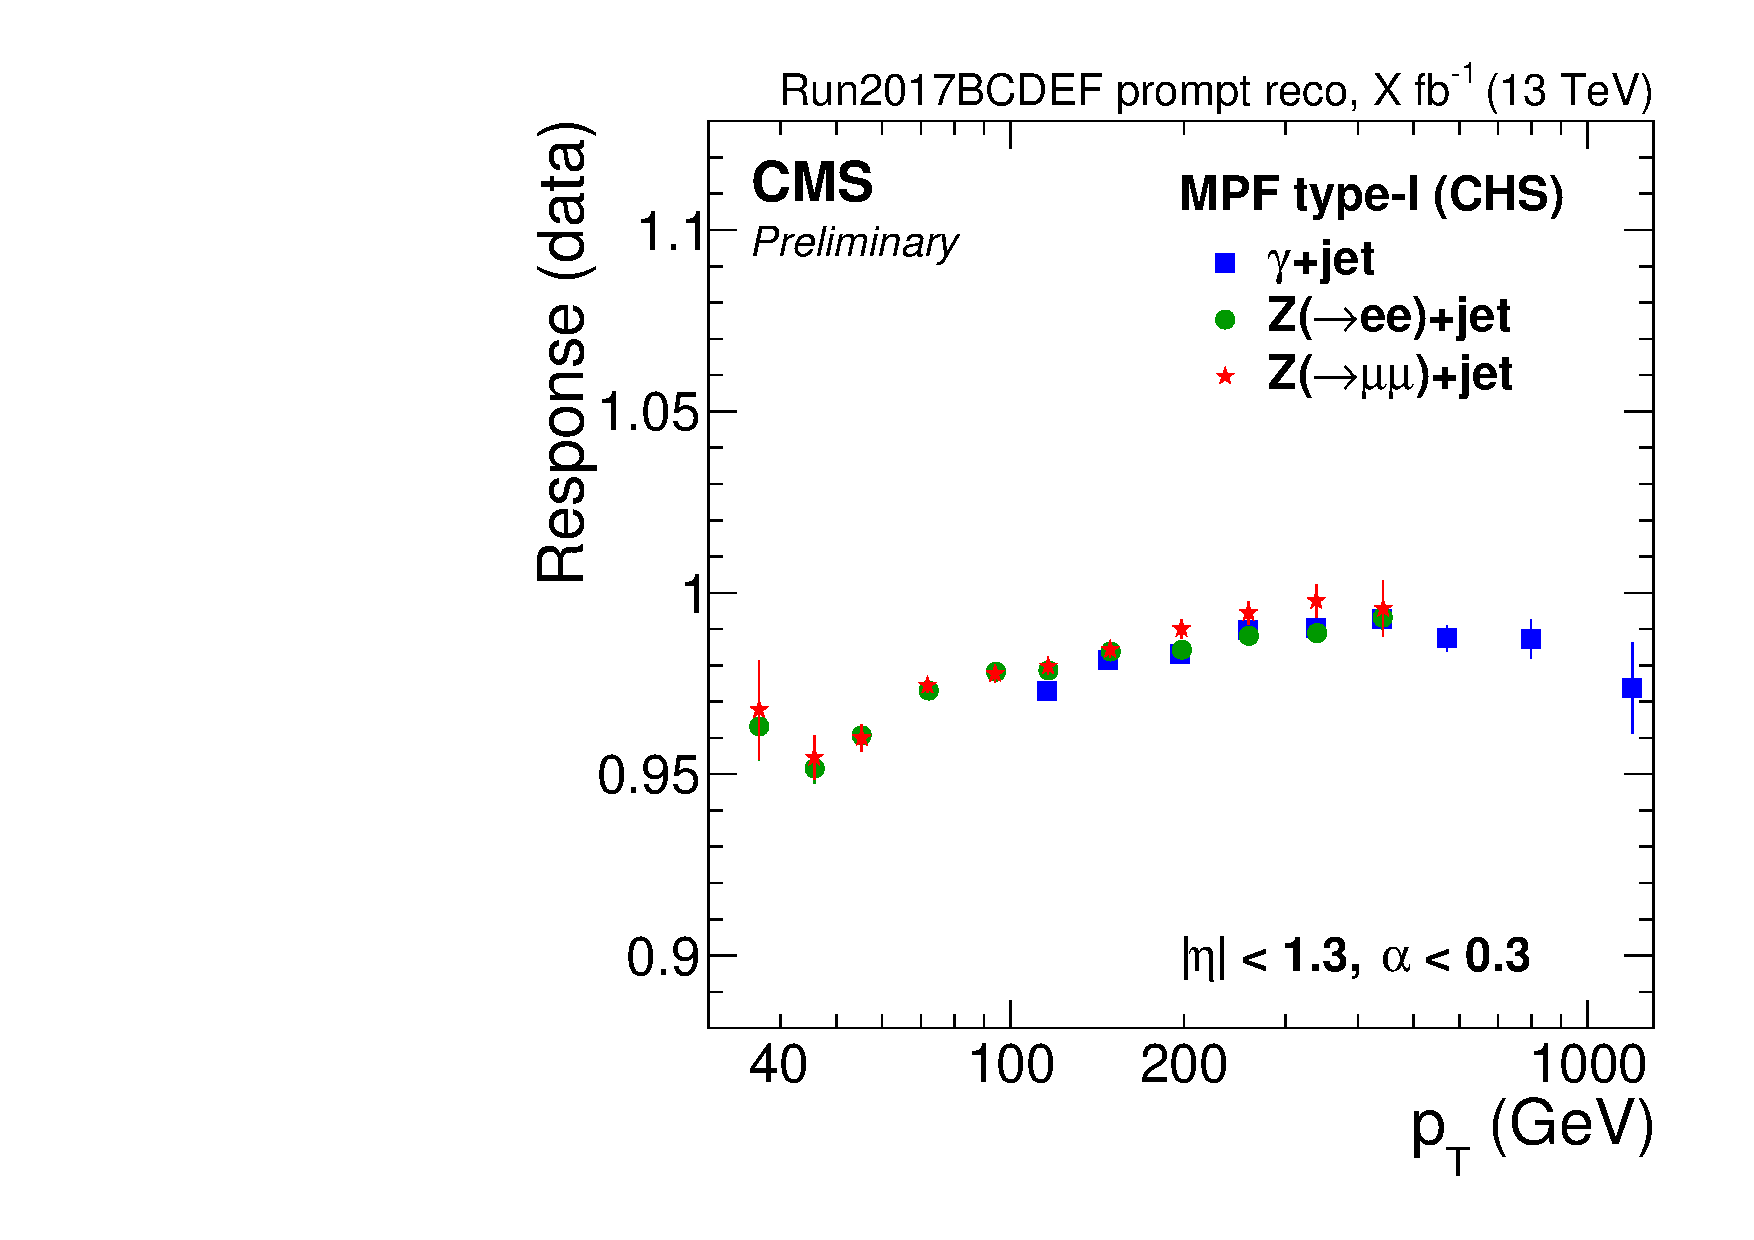
\includegraphics[width=0.10\textwidth]{\RunPeriod/paper_softrad_data_mpfchs1_vspt.pdf}
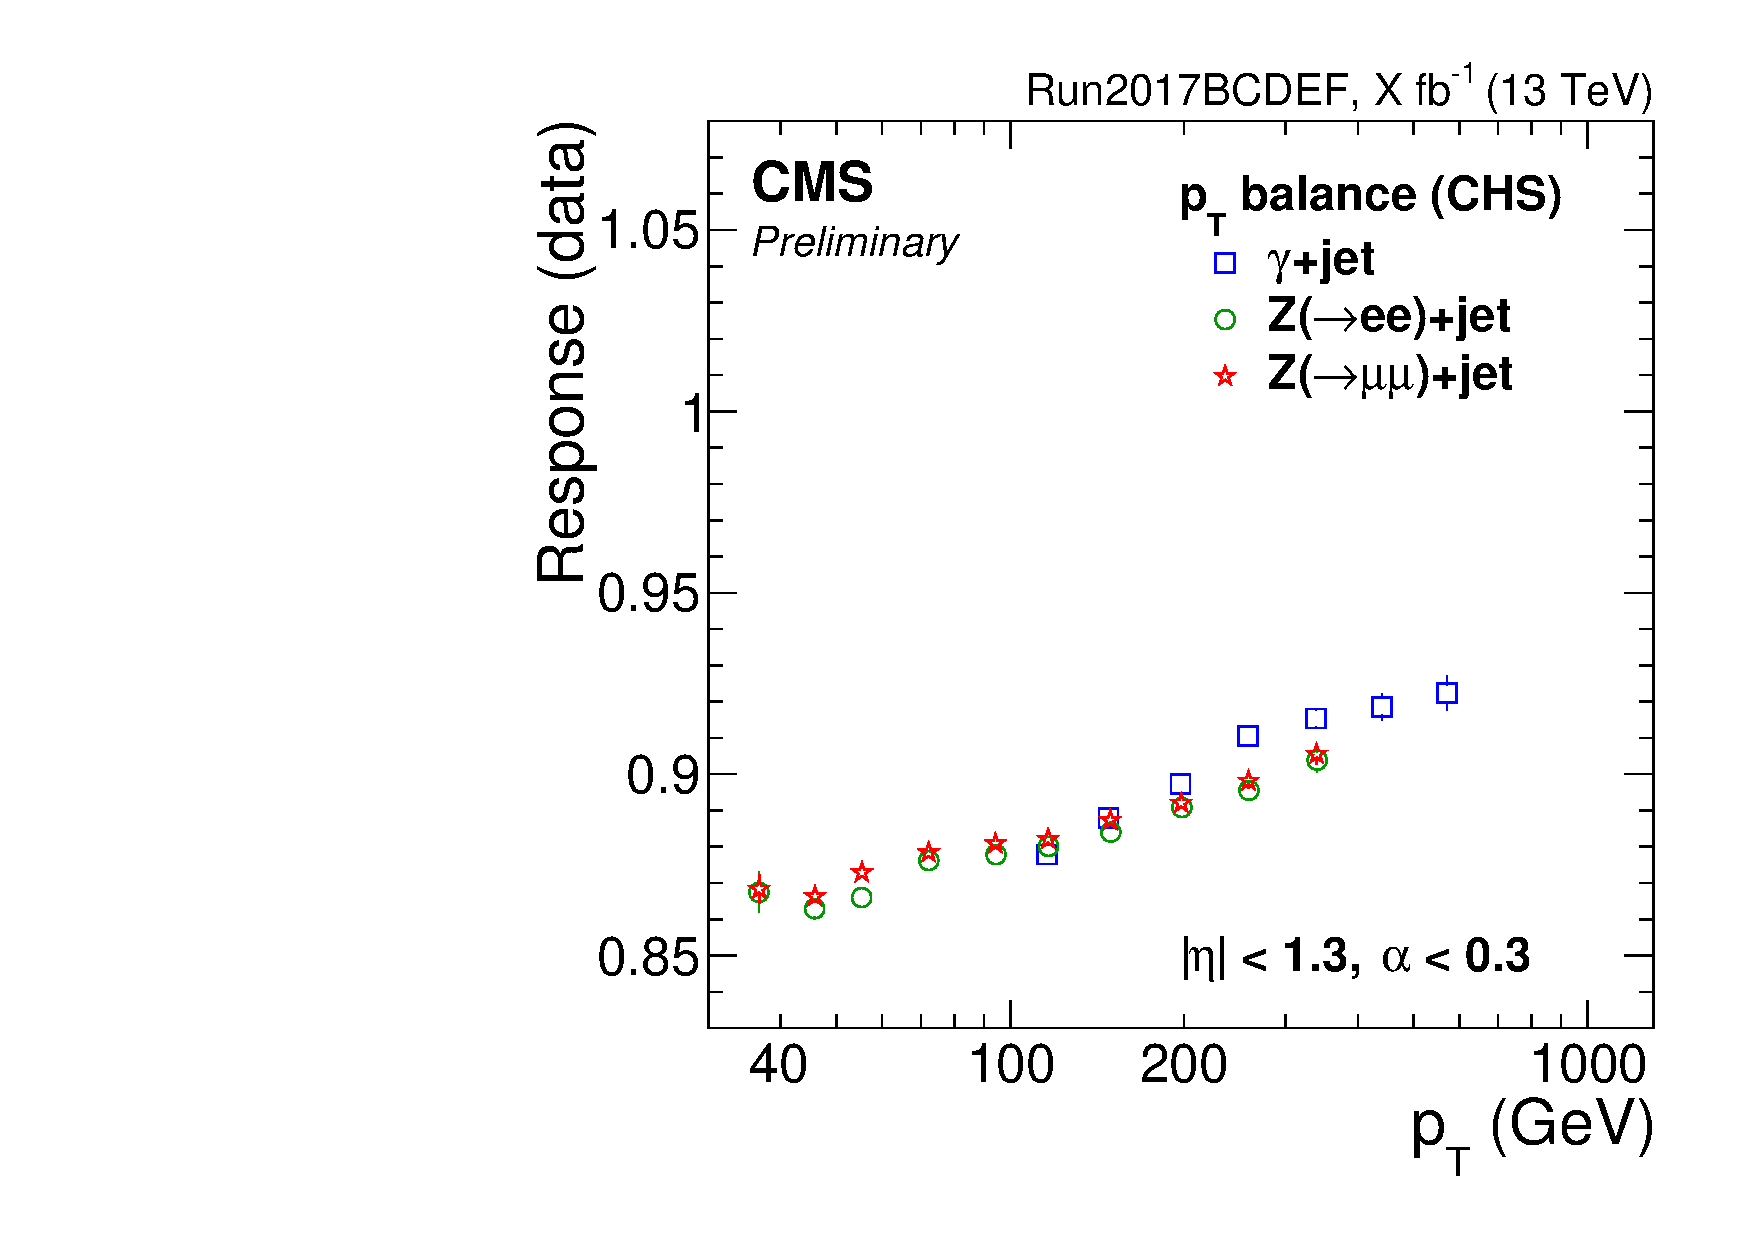
\includegraphics[width=0.10\textwidth]{\RunPeriod/paper_softrad_data_ptchs_vspt.pdf}
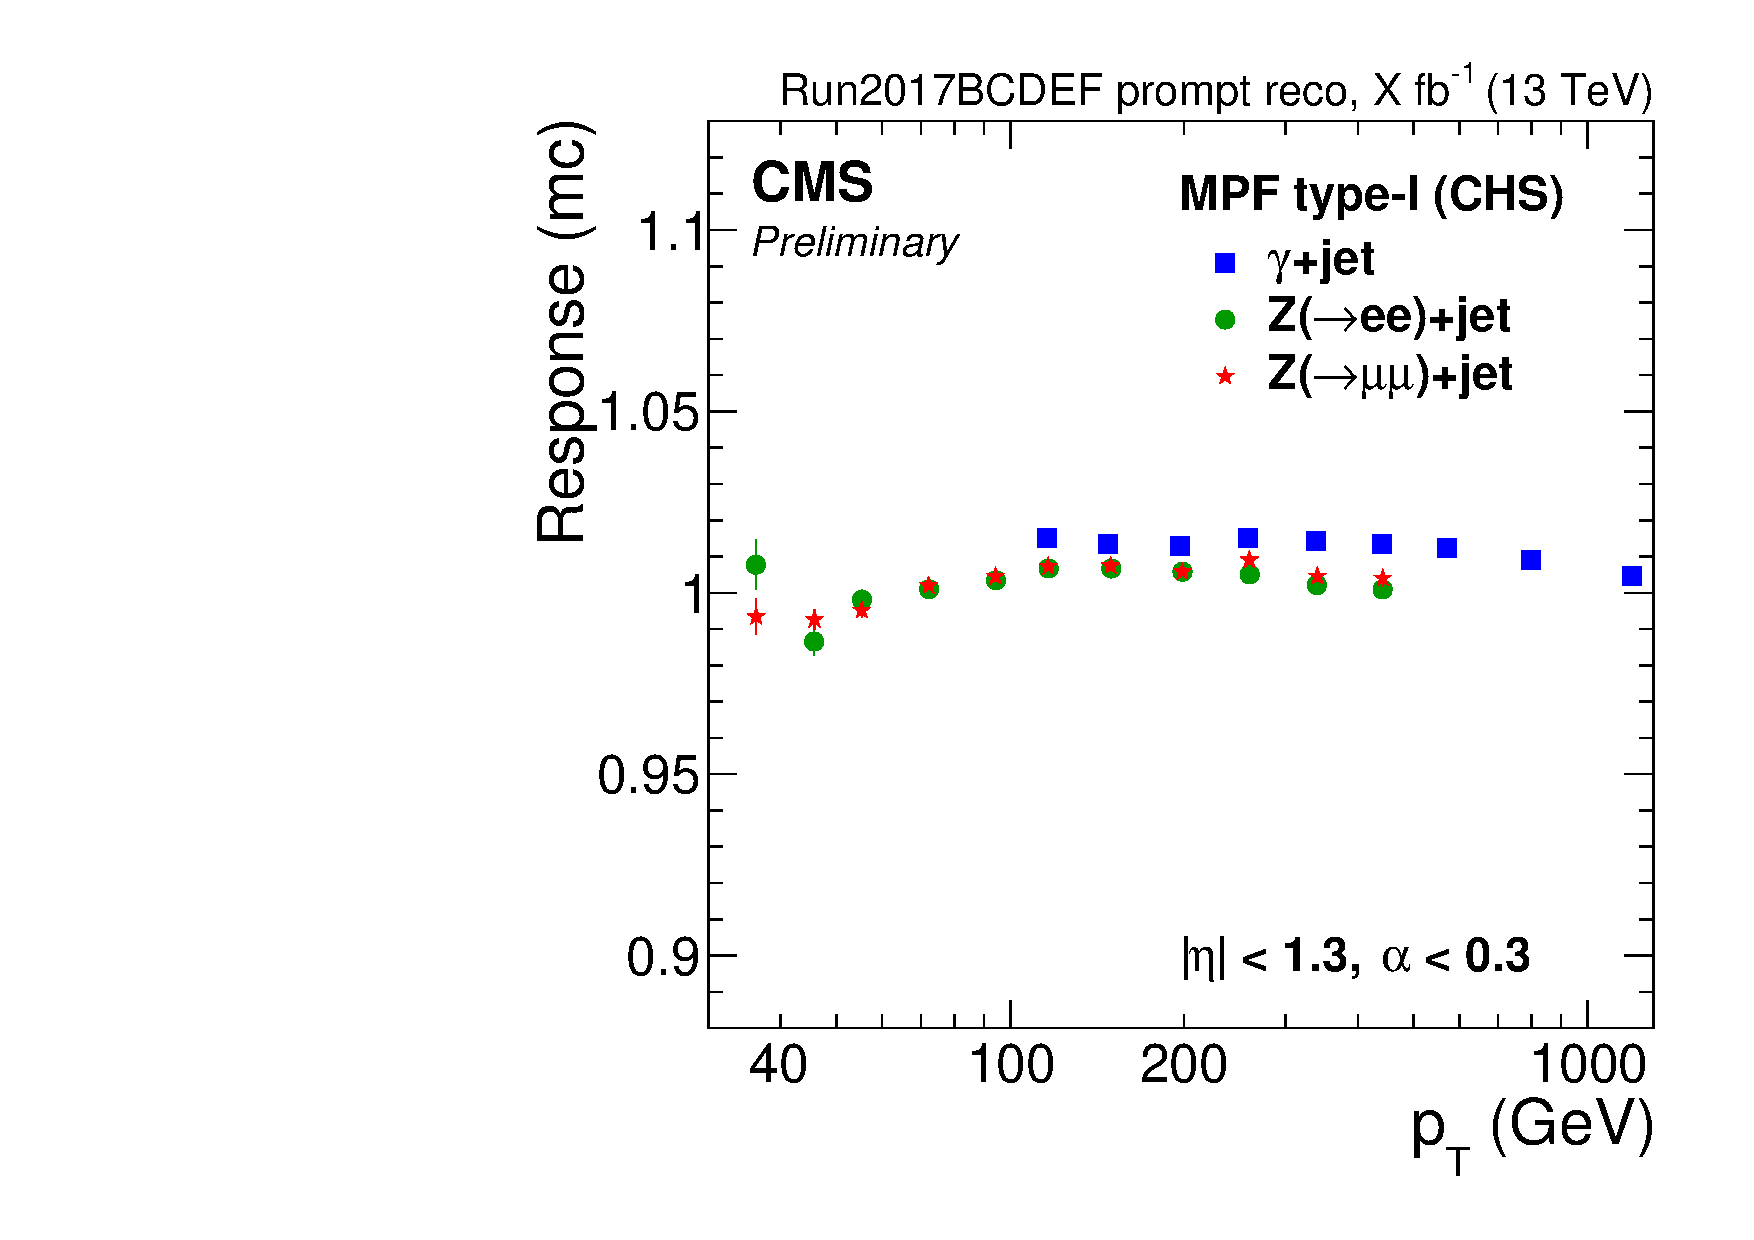
\includegraphics[width=0.10\textwidth]{\RunPeriod/paper_softrad_mc_mpfchs1_vspt.pdf}
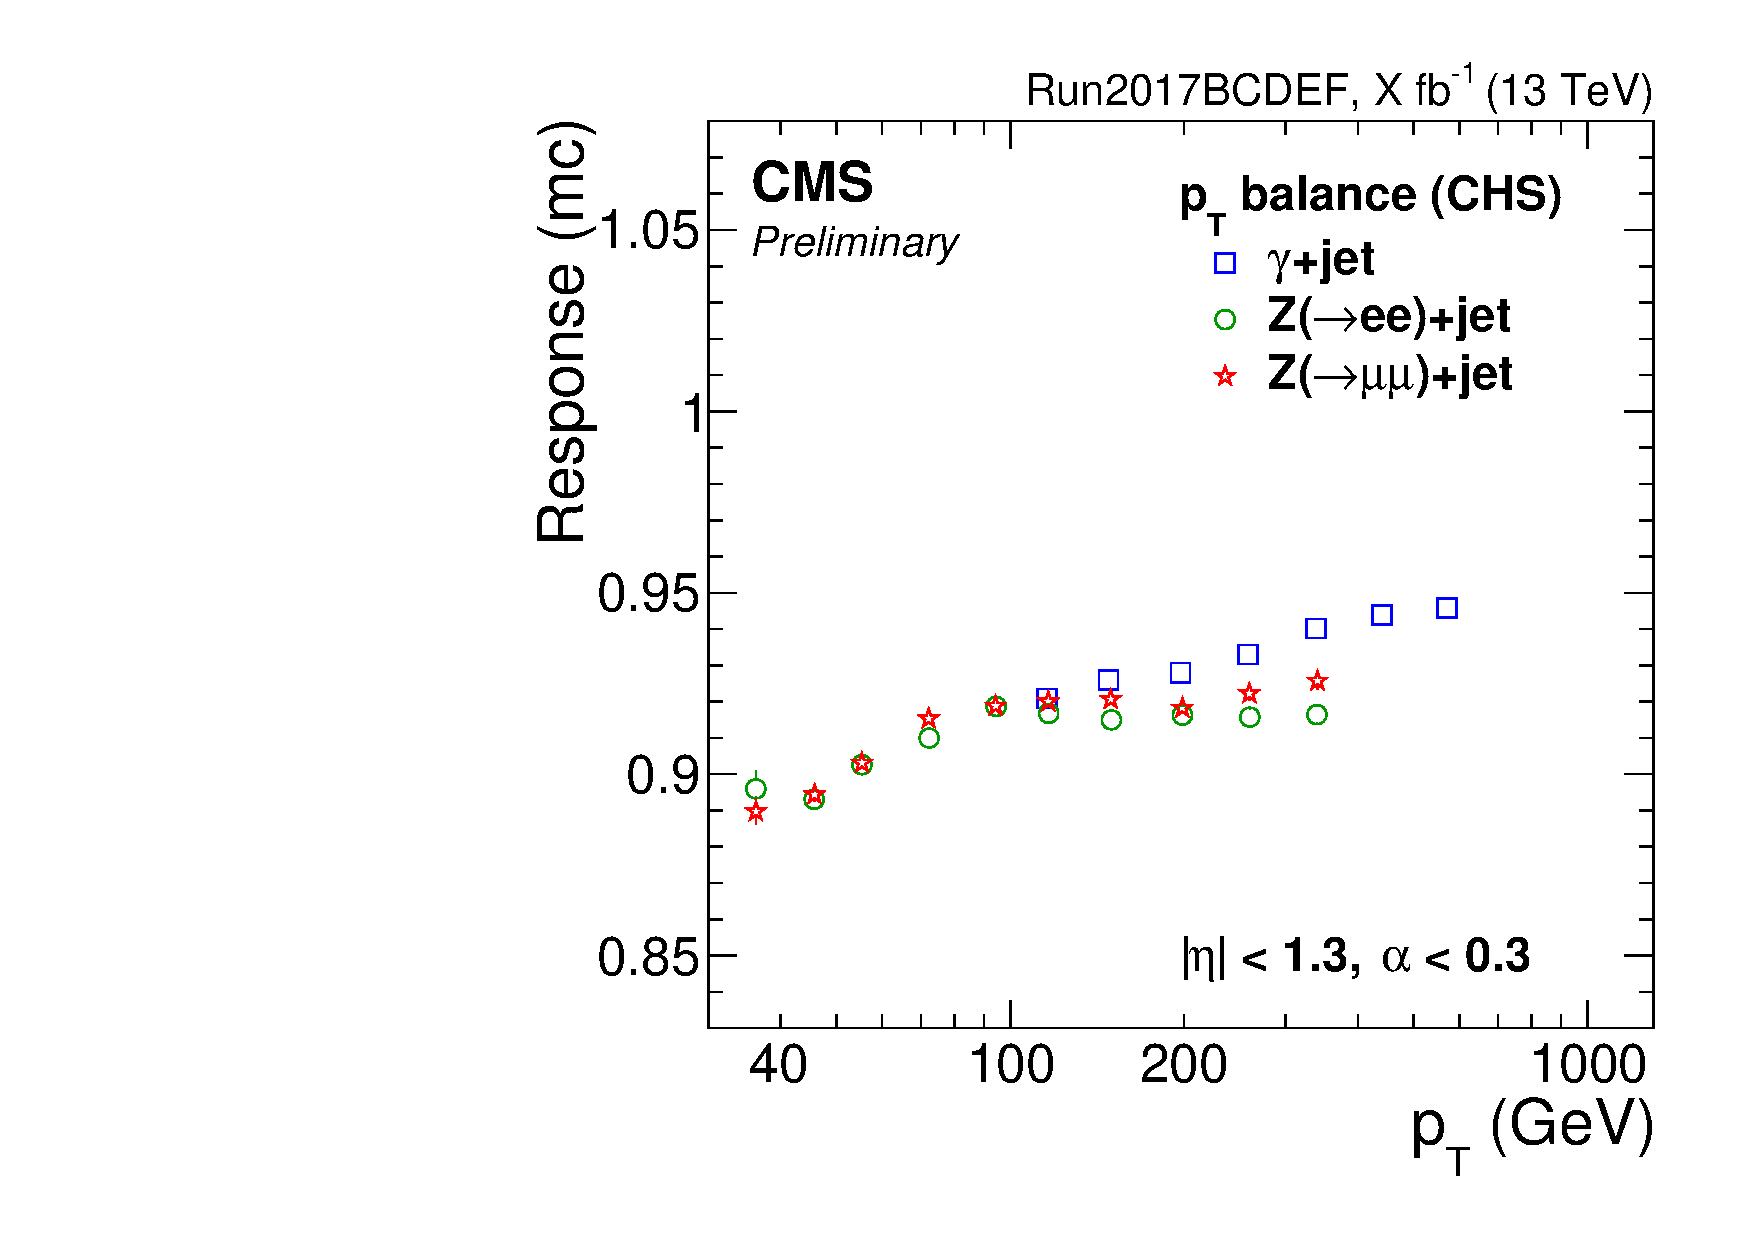
\includegraphics[width=0.10\textwidth]{\RunPeriod/paper_softrad_mc_ptchs_vspt.pdf}
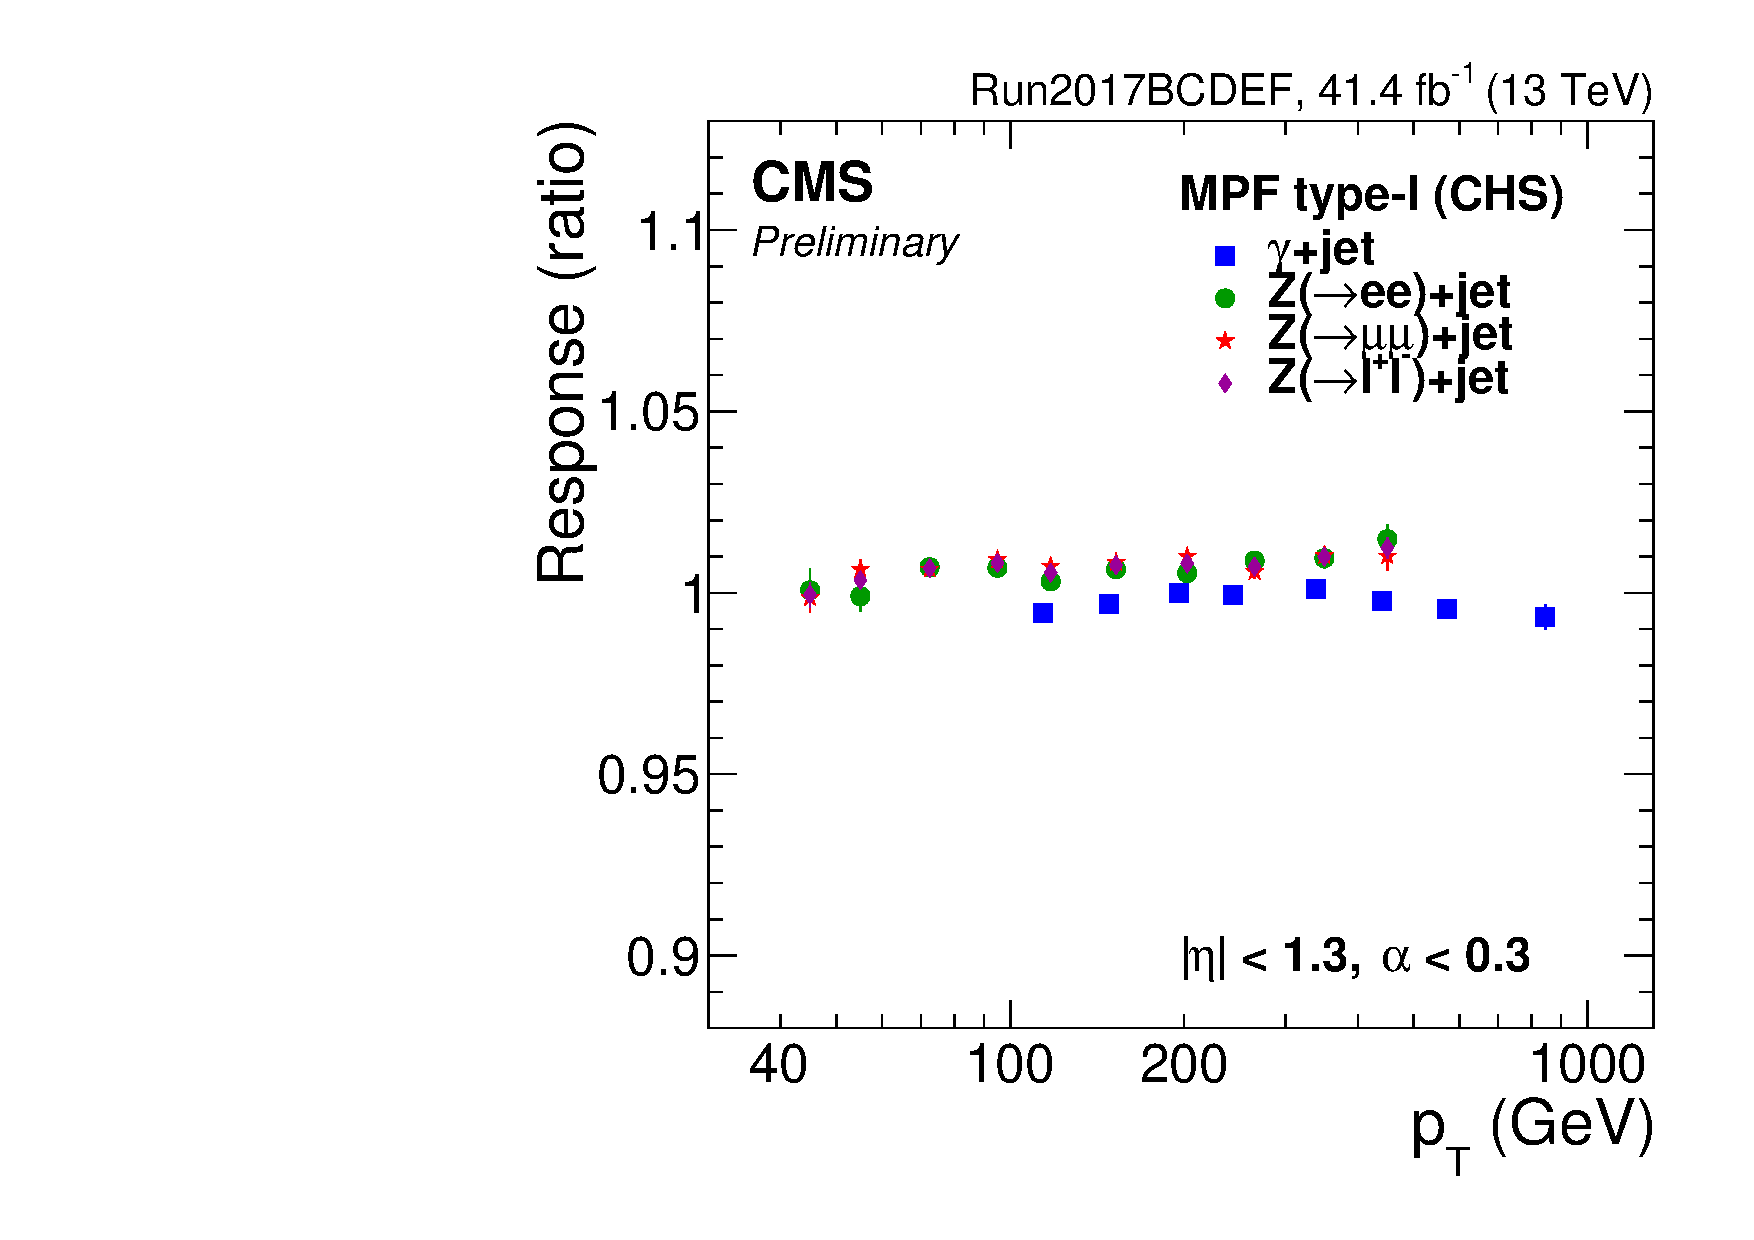
\includegraphics[width=0.10\textwidth]{\RunPeriod/paper_softrad_ratio_mpfchs1_vspt.pdf}
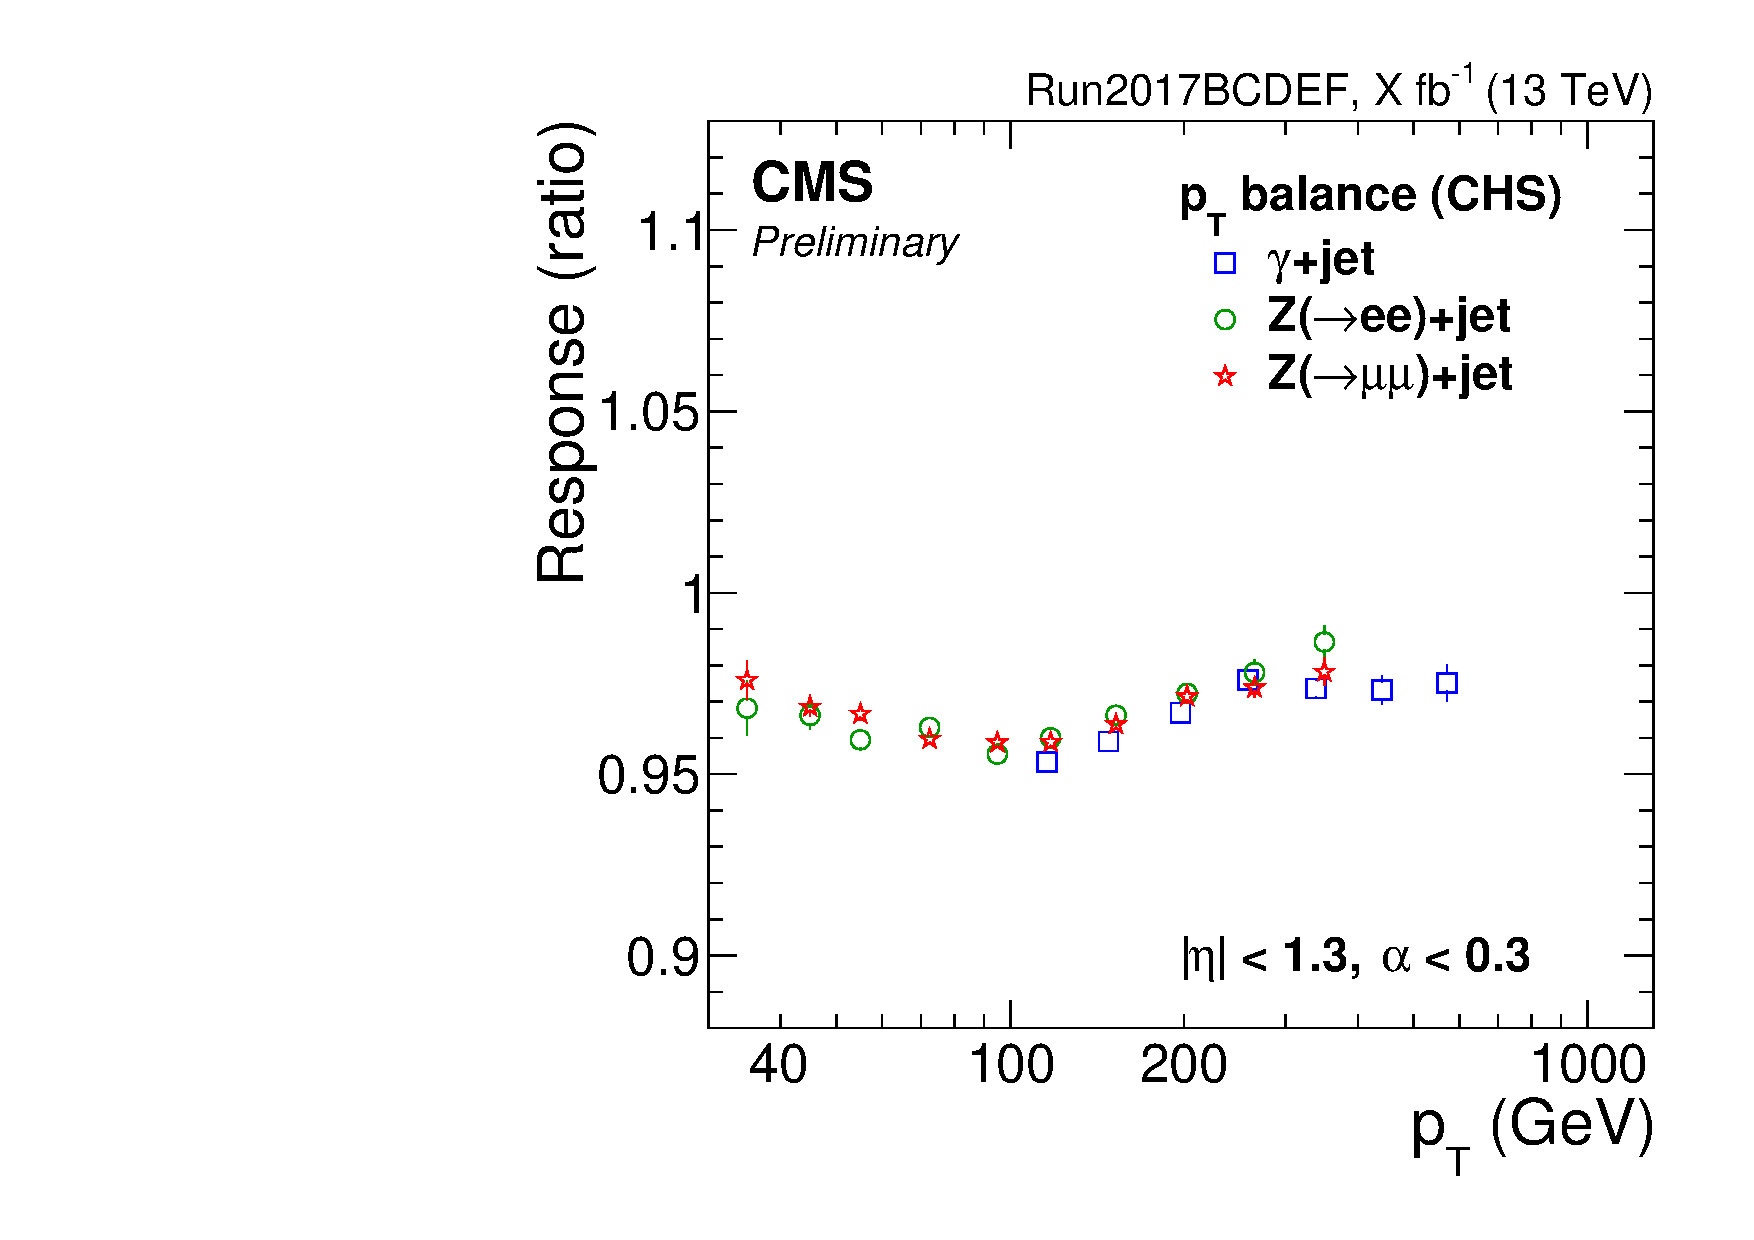
\includegraphics[width=0.10\textwidth]{\RunPeriod/paper_softrad_ratio_ptchs_vspt.pdf}



\foreach \n in \FineEtaBins{
  \newpage
%  \n \\
  \includegraphics[width=0.32\textwidth]{\RunPeriod/globalFitL3res_raw\n.pdf}
  \includegraphics[width=0.32\textwidth]{\RunPeriod/globalFitL3res_orig\n.pdf}
  \includegraphics[width=0.32\textwidth]{\RunPeriod/globalFitL3res_shifted\n.pdf}\\
  \includegraphics[width=0.30\textwidth]{\RunPeriod/softrad_2x6_kfsr\n.pdf}
  \includegraphics[width=0.30\textwidth]{\RunPeriod/softrad_2x6_vspt\n.pdf}
  \includegraphics[width=0.20\textwidth]{\RunPeriod/softrad_3x3_ratio_mpfchs1_vsalpha\n.pdf}
  \includegraphics[width=0.20\textwidth]{\RunPeriod/softrad_3x3_ratio_ptchs_vsalpha\n.pdf}\\

  \includegraphics[width=0.15\textwidth]{\RunPeriod/softrad_3x3_data_mpfchs1_vsalpha\n.pdf}
  \includegraphics[width=0.15\textwidth]{\RunPeriod/softrad_3x3_data_ptchs_vsalpha\n.pdf}
  \includegraphics[width=0.15\textwidth]{\RunPeriod/softrad_3x3_mc_mpfchs1_vsalpha\n.pdf} 
  \includegraphics[width=0.15\textwidth]{\RunPeriod/softrad_3x3_mc_ptchs_vsalpha\n.pdf}  
  \includegraphics[width=0.10\textwidth]{\RunPeriod/globalFitL3res_hsrc\n.pdf}
  \includegraphics[width=0.10\textwidth]{\RunPeriod/globalFitL3res_mpfchs1_kfsr\n.pdf}
  \includegraphics[width=0.10\textwidth]{\RunPeriod/globalFitL3res_ptchs_kfsr\n.pdf}\\

  \includegraphics[width=0.10\textwidth]{\RunPeriod/an_softrad_data_mpfchs1\n_vspt.pdf}
  \includegraphics[width=0.10\textwidth]{\RunPeriod/an_softrad_data_ptchs\n_vspt.pdf}
  \includegraphics[width=0.10\textwidth]{\RunPeriod/an_softrad_mc_mpfchs1\n_vspt.pdf}
  \includegraphics[width=0.10\textwidth]{\RunPeriod/an_softrad_mc_ptchs\n_vspt.pdf}
  \includegraphics[width=0.10\textwidth]{\RunPeriod/an_softrad_ratio_mpfchs1\n_vspt.pdf}
  \includegraphics[width=0.10\textwidth]{\RunPeriod/an_softrad_ratio_ptchs\n_vspt.pdf}


}


\newpage


\end{document}
